% !TeX program = XeLaTeX
% Working paper: benefit-cost analysis of MMC service delivery policies.
% Tables, figures and the numbers in the
% text (numbers.tex) are written by paper/make_paper.R from the model the app runs.
% Build: bash paper/build.sh draft   (or mac, on the Mac only)
\documentclass[11pt]{article}
\usepackage[letterpaper,margin=1.05in]{geometry}
\usepackage{amsthm}
\usepackage{amsmath,amssymb}
\usepackage[no-math]{fontspec}
\usepackage{mathspec}
\input{fonts}                      % fonts_mac.tex or fonts_draft.tex, copied to fonts.tex
\usepackage{xcolor}
\definecolor{secred}{RGB}{158,24,24}            % heading and link colour
% Okabe-Ito palette for figures and boxes
\definecolor{OIorange}{HTML}{E69F00}\definecolor{OIsky}{HTML}{56B4E9}
\definecolor{OIgreen}{HTML}{009E73}\definecolor{OIyellow}{HTML}{F0E442}
\definecolor{OIblue}{HTML}{0072B2}\definecolor{OIverm}{HTML}{D55E00}
\definecolor{OIpurple}{HTML}{CC79A7}\definecolor{OIgrey}{HTML}{999999}
\usepackage{graphicx,booktabs,array,tabularx,enumitem,titlesec,float,microtype}
\usepackage{threeparttable,multirow,makecell,adjustbox}
\usepackage[section]{placeins}
\setlength{\emergencystretch}{2em}   % loosen a line rather than let it run into the margin
\usepackage[super,sort&compress,comma]{natbib}
\usepackage[font={sf,small},labelfont=bf,labelsep=period,singlelinecheck=false]{caption}
\usepackage[colorlinks=true,linkcolor=secred,citecolor=secred,urlcolor=secred]{hyperref}
\IfFileExists{xurl.sty}{\usepackage{xurl}}{% URLs may break at any character; older TeX installs lack xurl,
  \expandafter\def\expandafter\UrlBreaks\expandafter{\UrlBreaks% so do what it does with url.sty
    \do\a\do\b\do\c\do\d\do\e\do\f\do\g\do\h\do\i\do\j\do\k\do\l\do\m\do\n\do\o\do\p\do\q\do\r\do\s\do\t\do\u\do\v\do\w\do\x\do\y\do\z
    \do\A\do\B\do\C\do\D\do\E\do\F\do\G\do\H\do\I\do\J\do\K\do\L\do\M\do\N\do\O\do\P\do\Q\do\R\do\S\do\T\do\U\do\V\do\W\do\X\do\Y\do\Z
    \do0\do1\do2\do3\do4\do5\do6\do7\do8\do9}}
\linespread{1.12}
\setlength{\parindent}{10pt}\setlength{\parskip}{2pt}
\frenchspacing \widowpenalty=10000 \clubpenalty=10000
\titleformat{\section}{\color{secred}\Large\scshape}{\thesection}{0.8em}{}
\titleformat{\subsection}{\color{secred}\large\scshape}{\thesubsection}{0.8em}{}
\titleformat{\subsubsection}{\itshape}{\thesubsubsection}{0.8em}{}
\numberwithin{equation}{section}\numberwithin{figure}{section}\numberwithin{table}{section}
\renewcommand{\cellalign}{cc}

\newcommand{\mmclambda}{0.0272}
\newcommand{\mmclambdaSE}{0.0052}
\newcommand{\mmcaHat}{2.924}
\newcommand{\mmcoptoutShare}{69.2}
\newcommand{\mmcuncalUptake}{89}
\newcommand{\mmctxPerMMC}{559}
\newcommand{\mmccashConst}{14}
\newcommand{\mmcvoucherConst}{7}
\newcommand{\mmcpctDroppedThree}{2.0}
\newcommand{\mmccostPerMMCmin}{48}
\newcommand{\mmccostPerMMCmax}{78}
\newcommand{\mmcPOneUptake}{43.4}
\newcommand{\mmcPOneUptakeChange}{12.6}
\newcommand{\mmcPOneCV}{\$7.39}
\newcommand{\mmcPOneCVlo}{\$5.20}
\newcommand{\mmcPOneCVhi}{\$12.07}
\newcommand{\mmcPOneCost}{\$9.83}
\newcommand{\mmcPOneTransfers}{\$0.00}
\newcommand{\mmcPOneNBcv}{$-$\$2.44}
\newcommand{\mmcPOneNBcvP}{9\%}
\newcommand{\mmcPOneTx}{\$70.52}
\newcommand{\mmcPOneNBtotal}{\$68.09}
\newcommand{\mmcPOneCostPerMMC}{\$78}
\newcommand{\mmcPOnePSAnbcv}{$-$\$2.05}
\newcommand{\mmcPOnePSAnbcvP}{13\%}
\newcommand{\mmcPOnePSAnbcvLo}{$-$\$5.15}
\newcommand{\mmcPOnePSAnbcvHi}{\$2.31}
\newcommand{\mmcPOneBestCV}{0\%}
\newcommand{\mmcPOneBestTotal}{0\%}
\newcommand{\mmcPOneCVthree}{\$7.38}
\newcommand{\mmcPOneCVthreeLo}{\$3.74}
\newcommand{\mmcPOneCVthreeHi}{\$41.09}
\newcommand{\mmcPTwoUptake}{41.3}
\newcommand{\mmcPTwoUptakeChange}{10.5}
\newcommand{\mmcPTwoCV}{\$6.04}
\newcommand{\mmcPTwoCVlo}{\$4.30}
\newcommand{\mmcPTwoCVhi}{\$9.62}
\newcommand{\mmcPTwoCost}{\$5.08}
\newcommand{\mmcPTwoTransfers}{\$0.00}
\newcommand{\mmcPTwoNBcv}{\$0.95}
\newcommand{\mmcPTwoNBcvP}{83\%}
\newcommand{\mmcPTwoTx}{\$58.65}
\newcommand{\mmcPTwoNBtotal}{\$59.60}
\newcommand{\mmcPTwoCostPerMMC}{\$48}
\newcommand{\mmcPTwoPSAnbcv}{\$1.35}
\newcommand{\mmcPTwoPSAnbcvP}{86\%}
\newcommand{\mmcPTwoPSAnbcvLo}{$-$\$0.79}
\newcommand{\mmcPTwoPSAnbcvHi}{\$4.82}
\newcommand{\mmcPTwoBestCV}{31\%}
\newcommand{\mmcPTwoBestTotal}{0\%}
\newcommand{\mmcPTwoCVthree}{\$5.97}
\newcommand{\mmcPTwoCVthreeLo}{\$2.98}
\newcommand{\mmcPTwoCVthreeHi}{\$34.27}
\newcommand{\mmcPThreeUptake}{50.6}
\newcommand{\mmcPThreeUptakeChange}{19.8}
\newcommand{\mmcPThreeCV}{\$12.40}
\newcommand{\mmcPThreeCVlo}{\$8.91}
\newcommand{\mmcPThreeCVhi}{\$19.78}
\newcommand{\mmcPThreeCost}{\$12.85}
\newcommand{\mmcPThreeTransfers}{\$0.00}
\newcommand{\mmcPThreeNBcv}{$-$\$0.45}
\newcommand{\mmcPThreeNBcvP}{42\%}
\newcommand{\mmcPThreeTx}{\$110.86}
\newcommand{\mmcPThreeNBtotal}{\$110.41}
\newcommand{\mmcPThreeCostPerMMC}{\$65}
\newcommand{\mmcPThreePSAnbcv}{\$0.25}
\newcommand{\mmcPThreePSAnbcvP}{48\%}
\newcommand{\mmcPThreePSAnbcvLo}{$-$\$4.16}
\newcommand{\mmcPThreePSAnbcvHi}{\$7.22}
\newcommand{\mmcPThreeBestCV}{0\%}
\newcommand{\mmcPThreeBestTotal}{0\%}
\newcommand{\mmcPThreeCVthree}{\$12.32}
\newcommand{\mmcPThreeCVthreeLo}{\$6.27}
\newcommand{\mmcPThreeCVthreeHi}{\$69.27}
\newcommand{\mmcPFourUptake}{57.2}
\newcommand{\mmcPFourUptakeChange}{26.5}
\newcommand{\mmcPFourCV}{\$17.70}
\newcommand{\mmcPFourCVlo}{\$12.76}
\newcommand{\mmcPFourCVhi}{\$28.15}
\newcommand{\mmcPFourCost}{\$16.97}
\newcommand{\mmcPFourTransfers}{\$5.48}
\newcommand{\mmcPFourNBcv}{\$0.73}
\newcommand{\mmcPFourNBcvP}{59\%}
\newcommand{\mmcPFourTx}{\$147.94}
\newcommand{\mmcPFourNBtotal}{\$148.67}
\newcommand{\mmcPFourCostPerMMC}{\$64}
\newcommand{\mmcPFourPSAnbcv}{\$1.66}
\newcommand{\mmcPFourPSAnbcvP}{63\%}
\newcommand{\mmcPFourPSAnbcvLo}{$-$\$4.05}
\newcommand{\mmcPFourPSAnbcvHi}{\$11.57}
\newcommand{\mmcPFourBestCV}{6\%}
\newcommand{\mmcPFourBestTotal}{0\%}
\newcommand{\mmcPFourCVthree}{\$18.17}
\newcommand{\mmcPFourCVthreeLo}{\$9.97}
\newcommand{\mmcPFourCVthreeHi}{\$94.17}
\newcommand{\mmcPFiveUptake}{62.4}
\newcommand{\mmcPFiveUptakeChange}{31.6}
\newcommand{\mmcPFiveCV}{\$22.44}
\newcommand{\mmcPFiveCVlo}{\$16.26}
\newcommand{\mmcPFiveCVhi}{\$35.52}
\newcommand{\mmcPFiveCost}{\$21.45}
\newcommand{\mmcPFiveTransfers}{\$4.81}
\newcommand{\mmcPFiveNBcv}{\$0.99}
\newcommand{\mmcPFiveNBcvP}{60\%}
\newcommand{\mmcPFiveTx}{\$176.88}
\newcommand{\mmcPFiveNBtotal}{\$177.87}
\newcommand{\mmcPFiveCostPerMMC}{\$68}
\newcommand{\mmcPFivePSAnbcv}{\$2.15}
\newcommand{\mmcPFivePSAnbcvP}{63\%}
\newcommand{\mmcPFivePSAnbcvLo}{$-$\$5.04}
\newcommand{\mmcPFivePSAnbcvHi}{\$14.58}
\newcommand{\mmcPFiveBestCV}{49\%}
\newcommand{\mmcPFiveBestTotal}{100\%}
\newcommand{\mmcPFiveCVthree}{\$22.81}
\newcommand{\mmcPFiveCVthreeLo}{\$12.37}
\newcommand{\mmcPFiveCVthreeHi}{\$120.45}
\newcommand{\mmcInitBestCV}{14\%}
\newcommand{\mmcOWcvTopOne}{price}
\newcommand{\mmcOWcvTopOneLo}{$-$\$4.66}
\newcommand{\mmcOWcvTopOneHi}{\$12.50}
\newcommand{\mmcOWcvTopTwo}{share who stay uncircumcised, initial state}
\newcommand{\mmcOWcvTopThree}{device circumcision at permanent health facilities, per procedure}
\newcommand{\mmcOWtotTop}{circumcisions per hiv infection averted; years on art per averted infection; discount rate for averted treatment costs; antiretroviral therapy (art), cost per person per year}
\newcommand{\mmcReproOutreach}{\$27.29}
\newcommand{\mmcReproDevice}{\$14.80}
\newcommand{\mmcReproCash}{\$44.71}
\newcommand{\mmcMXdraws}{3,000}
\newcommand{\mmcMXsimMen}{2,000}
\newcommand{\mmcMXkr}{200}
\newcommand{\mmcMXstarts}{1}
\newcommand{\mmcMXllFixed}{$-$2,721.5}
\newcommand{\mmcMXbicFixed}{5,621.3}
\newcommand{\mmcMXgainFixed}{982}
\newcommand{\mmcMXllThreeFixed}{$-$2,721.8}
\newcommand{\mmcMXbicThreeFixed}{5,638.8}
\newcommand{\mmcMXllLogn}{$-$2,683.8}
\newcommand{\mmcMXbicLogn}{5,554.5}
\newcommand{\mmcMXgainLogn}{1,019}
\newcommand{\mmcMXllThreeLogn}{$-$2,688.6}
\newcommand{\mmcMXbicThreeLogn}{5,598.0}
\newcommand{\mmcMXllCens}{$-$2,685.3}
\newcommand{\mmcMXbicCens}{5,557.4}
\newcommand{\mmcMXgainCens}{1,018}
\newcommand{\mmcMXllThreeCens}{$-$2,692.8}
\newcommand{\mmcMXbicThreeCens}{5,606.5}
\newcommand{\mmcMXgainPrice}{38}
\newcommand{\mmcMXpriceFixed}{$-$0.0510}
\newcommand{\mmcMXscale}{1.9}
\newcommand{\mmcMXneitherSD}{2.97}
\newcommand{\mmcMXpermhcMean}{2.00}
\newcommand{\mmcMXpermhcSD}{1.53}
\newcommand{\mmcMXdeviceMean}{$-$1.61}
\newcommand{\mmcMXdeviceSD}{3.61}
\newcommand{\mmcMXdeviceLike}{33\%}
\newcommand{\mmcMXcashMean}{0.95}
\newcommand{\mmcMXcashSD}{0.97}
\newcommand{\mmcMXlognMedian}{$-$0.0229}
\newcommand{\mmcMXlognMean}{$-$0.1703}
\newcommand{\mmcMXlognRatio}{7.4}
\newcommand{\mmcMXcensZero}{67\%}
\newcommand{\mmcMXPOneUptake}{36.8}
\newcommand{\mmcMXPOneCV}{\$3.50}
\newcommand{\mmcMXPOneCVlo}{\$2.47}
\newcommand{\mmcMXPOneCVhi}{\$6.03}
\newcommand{\mmcMXPOneCVmed}{\$0.85}
\newcommand{\mmcMXPOneCost}{\$5.89}
\newcommand{\mmcMXPOneNB}{$-$\$2.39}
\newcommand{\mmcMXPOneNBlo}{$-$\$3.52}
\newcommand{\mmcMXPOneNBhi}{\$0.06}
\newcommand{\mmcMXPOneGain}{18\%}
\newcommand{\mmcMXPOneNBtotal}{\$31.61}
\newcommand{\mmcMXPOnePlugFixed}{\$2.56}
\newcommand{\mmcMXPOneCVLogn}{\$93}
\newcommand{\mmcMXPOneCVmedLogn}{\$1.43}
\newcommand{\mmcMXPOnePlugLogn}{\$5.95}
\newcommand{\mmcMXPOneGainLogn}{33\%}
\newcommand{\mmcMXPOneCVloLogn}{\$22}
\newcommand{\mmcMXPOneCVhiLogn}{\$644}
\newcommand{\mmcMXPOneCVCens}{\$25}
\newcommand{\mmcMXPOneCVmedCens}{\$0.18}
\newcommand{\mmcMXPOnePlugCens}{\$43.12}
\newcommand{\mmcMXPOneGainCens}{10\%}
\newcommand{\mmcMXPOneCVloCens}{\$1}
\newcommand{\mmcMXPOneCVhiCens}{\$35}
\newcommand{\mmcMXPTwoUptake}{38.7}
\newcommand{\mmcMXPTwoCV}{\$7.01}
\newcommand{\mmcMXPTwoCVlo}{\$5.24}
\newcommand{\mmcMXPTwoCVhi}{\$12.13}
\newcommand{\mmcMXPTwoCVmed}{\$0.37}
\newcommand{\mmcMXPTwoCost}{\$4.16}
\newcommand{\mmcMXPTwoNB}{\$2.84}
\newcommand{\mmcMXPTwoNBlo}{\$0.86}
\newcommand{\mmcMXPTwoNBhi}{\$7.80}
\newcommand{\mmcMXPTwoGain}{23\%}
\newcommand{\mmcMXPTwoNBtotal}{\$47.22}
\newcommand{\mmcMXPTwoPlugFixed}{\$6.85}
\newcommand{\mmcMXPTwoCVLogn}{\$194}
\newcommand{\mmcMXPTwoCVmedLogn}{\$0.59}
\newcommand{\mmcMXPTwoPlugLogn}{\$11.61}
\newcommand{\mmcMXPTwoGainLogn}{31\%}
\newcommand{\mmcMXPTwoCVloLogn}{\$45}
\newcommand{\mmcMXPTwoCVhiLogn}{\$1,586}
\newcommand{\mmcMXPTwoCVCens}{\$7}
\newcommand{\mmcMXPTwoCVmedCens}{\$0.08}
\newcommand{\mmcMXPTwoPlugCens}{\$39.60}
\newcommand{\mmcMXPTwoGainCens}{13\%}
\newcommand{\mmcMXPTwoCVloCens}{\$2}
\newcommand{\mmcMXPTwoCVhiCens}{\$43}
\newcommand{\mmcMXPThreeUptake}{43.3}
\newcommand{\mmcMXPThreeCV}{\$9.77}
\newcommand{\mmcMXPThreeCVlo}{\$7.37}
\newcommand{\mmcMXPThreeCVhi}{\$16.80}
\newcommand{\mmcMXPThreeCVmed}{\$2.29}
\newcommand{\mmcMXPThreeCost}{\$8.71}
\newcommand{\mmcMXPThreeNB}{\$1.06}
\newcommand{\mmcMXPThreeNBlo}{$-$\$1.77}
\newcommand{\mmcMXPThreeNBhi}{\$8.02}
\newcommand{\mmcMXPThreeGain}{27\%}
\newcommand{\mmcMXPThreeNBtotal}{\$71.22}
\newcommand{\mmcMXPThreePlugFixed}{\$9.06}
\newcommand{\mmcMXPThreeCVLogn}{\$248}
\newcommand{\mmcMXPThreeCVmedLogn}{\$4.00}
\newcommand{\mmcMXPThreePlugLogn}{\$16.64}
\newcommand{\mmcMXPThreeGainLogn}{41\%}
\newcommand{\mmcMXPThreeCVloLogn}{\$59}
\newcommand{\mmcMXPThreeCVhiLogn}{\$1,897}
\newcommand{\mmcMXPThreeCVCens}{\$31}
\newcommand{\mmcMXPThreeCVmedCens}{\$0.57}
\newcommand{\mmcMXPThreePlugCens}{\$76.95}
\newcommand{\mmcMXPThreeGainCens}{13\%}
\newcommand{\mmcMXPThreeCVloCens}{\$3}
\newcommand{\mmcMXPThreeCVhiCens}{\$68}
\newcommand{\mmcMXPFourUptake}{53.8}
\newcommand{\mmcMXPFourCV}{\$21.10}
\newcommand{\mmcMXPFourCVlo}{\$14.98}
\newcommand{\mmcMXPFourCVhi}{\$37.11}
\newcommand{\mmcMXPFourCVmed}{\$9.94}
\newcommand{\mmcMXPFourCost}{\$15.28}
\newcommand{\mmcMXPFourNB}{\$5.82}
\newcommand{\mmcMXPFourNBlo}{$-$\$0.20}
\newcommand{\mmcMXPFourNBhi}{\$22.05}
\newcommand{\mmcMXPFourGain}{41\%}
\newcommand{\mmcMXPFourNBtotal}{\$134.81}
\newcommand{\mmcMXPFourPlugFixed}{\$21.83}
\newcommand{\mmcMXPFourCVLogn}{\$339}
\newcommand{\mmcMXPFourCVmedLogn}{\$13.03}
\newcommand{\mmcMXPFourPlugLogn}{\$27.25}
\newcommand{\mmcMXPFourGainLogn}{46\%}
\newcommand{\mmcMXPFourCVloLogn}{\$80}
\newcommand{\mmcMXPFourCVhiLogn}{\$2,574}
\newcommand{\mmcMXPFourCVCens}{\$81}
\newcommand{\mmcMXPFourCVmedCens}{\$7.24}
\newcommand{\mmcMXPFourPlugCens}{\$83.18}
\newcommand{\mmcMXPFourGainCens}{25\%}
\newcommand{\mmcMXPFourCVloCens}{\$9}
\newcommand{\mmcMXPFourCVhiCens}{\$119}
\newcommand{\mmcMXPFiveUptake}{56.2}
\newcommand{\mmcMXPFiveCV}{\$22.73}
\newcommand{\mmcMXPFiveCVlo}{\$16.25}
\newcommand{\mmcMXPFiveCVhi}{\$40.13}
\newcommand{\mmcMXPFiveCVmed}{\$12.63}
\newcommand{\mmcMXPFiveCost}{\$17.54}
\newcommand{\mmcMXPFiveNB}{\$5.19}
\newcommand{\mmcMXPFiveNBlo}{$-$\$1.39}
\newcommand{\mmcMXPFiveNBhi}{\$22.50}
\newcommand{\mmcMXPFiveGain}{43\%}
\newcommand{\mmcMXPFiveNBtotal}{\$147.49}
\newcommand{\mmcMXPFivePlugFixed}{\$22.97}
\newcommand{\mmcMXPFiveCVLogn}{\$372}
\newcommand{\mmcMXPFiveCVmedLogn}{\$16.67}
\newcommand{\mmcMXPFivePlugLogn}{\$30.69}
\newcommand{\mmcMXPFiveGainLogn}{49\%}
\newcommand{\mmcMXPFiveCVloLogn}{\$90}
\newcommand{\mmcMXPFiveCVhiLogn}{\$2,742}
\newcommand{\mmcMXPFiveCVCens}{\$94}
\newcommand{\mmcMXPFiveCVmedCens}{\$7.60}
\newcommand{\mmcMXPFivePlugCens}{\$113.89}
\newcommand{\mmcMXPFiveGainCens}{20\%}
\newcommand{\mmcMXPFiveCVloCens}{\$9}
\newcommand{\mmcMXPFiveCVhiCens}{\$123}
\newcommand{\mmcMXuptakeDiffMin}{3}
\newcommand{\mmcMXuptakeDiffMax}{7}
\newcommand{\mmcMXtxDrop}{20\%}
\newcommand{\mmcMXgainMin}{18\%}
\newcommand{\mmcMXgainMax}{43\%}
\newcommand{\mmcMXmedFiveMin}{\$7.60}
\newcommand{\mmcMXmedFiveMax}{\$16.67}
\newcommand{\mmcMXpopDiff}{23\%}
                    % numbers quoted in the text, from make_paper.R

\title{{\slabfont Preferences for medical male circumcision services and the benefits and costs of alternative service delivery policies: a discrete choice experiment among uncircumcised men in Uganda}}
\author{\textsf{Solomon J. Lubinga, Joseph B. Babigumira, Susan M. Graham,}\\
  \textsf{Aggrey D. Mukose, Louis P. Garrison Jr, Anirban Basu}\\[0.4em]
  \small\textsf{Working paper \textperiodcentered{} 1 November 2026}}
\date{}

\begin{document}
\maketitle
\thispagestyle{plain}

\begin{abstract}
\noindent Medical male circumcision (MMC) prevents HIV infection in men, but uptake in many priority countries has fallen short of targets. Discrete choice experiments (DCEs) are widely used to study the demand for health services, yet they are rarely used for what welfare economics allows them to do: value a policy in money, so that it can be weighed against what it costs. We conducted a DCE among 406 uncircumcised, HIV-negative men aged 18--45 years in a fishing community in Uganda with high HIV prevalence, and used it to value five policies to increase the uptake of MMC: outreach services, device circumcision, both together, cash incentives, and cash incentives with outreach services. We estimated conditional and mixed logit models, calibrated them to the observed share of uncircumcised men, and computed the compensating variation (CV) of each policy, which we compared with the incremental cost of the services and incentives and with the HIV treatment costs averted by additional circumcisions. With the conditional logit, the CV of every policy was within \$2.50 of its cost per man. Outreach services were worth less to men than they cost, while device circumcision and cash incentives were worth slightly more. Cash incentives with outreach services raised uptake the most, to \mmcPFiveUptake\%, and had the highest CV, \mmcPFiveCV{} per uncircumcised man. Once averted treatment costs were counted, every policy had a large positive net benefit. Seen from the health budget, each dollar spent on additional circumcisions saved \mmcBreturnMin{} to \mmcBreturnMax{} dollars in future HIV treatment costs, an internal rate of return of \mmcBirrMin{} to \mmcBirrMax{} a year, although it took six to seven years to recover the cost. The mixed logits fitted the data far better. With a fixed price coefficient, they led to the same conclusions for four of the five policies, but they showed that the value of each policy was concentrated in a minority of men: fewer than half valued any policy at more than its cost. When the marginal utility of income was allowed to vary across men, the mean CV was dominated by men who were almost indifferent to price, while the median was far less sensitive. DCEs can supply the benefit side of a benefit-cost analysis, provided the marginal utility of income is well determined and the model is calibrated to observed uptake. With external funding for MMC withdrawn, these returns make a strong case for governments to fund MMC at permanent health facilities from their own budgets.
\end{abstract}

{\small\textbf{Keywords:} Medical Male Circumcision; Discrete choice experiment; Compensating variation; Mixed logit; Benefit-cost analysis \\
\textbf{JEL Codes:} C35; D61; I12; I18}


\section{Introduction}
Medical Male Circumcision (MMC) of adolescent boys and men is an effective intervention for the prevention of female-to-male HIV transmission.\cite{RN16} Njeuhmeli et al.,\cite{RN25} projected a potentially high return-on-investment from scaling-up MMC to 80\% coverage in 13 priority-countries in sub-Saharan Africa with high-HIV and low-circumcision prevalence. In 2011, the WHO/UNAIDS set a target of performing 20.3 million circumcisions in the priority countries by 2016. However, by 2015, an estimated 11.7 million adolescent boys and men had been circumcised, representing 58\% of this target.\cite{RN94} Since the cuts in United States funding in 2025, programmes have contracted sharply: in Uganda, circumcisions fell by 65\% in the first half of 2025.\cite{UNAIDS2025,Devex2025}

Economic evaluations have shown that MMC is highly cost-effective when compared to no MMC,\cite{RN17,RN18,RN19,RN20,RN21} and a portfolio of biomedical HIV prevention interventions.\cite{RN23} However, qualitative studies have documented intangible (psychological and socio-cultural) costs that impede acceptability of circumcision,\cite{RN173} and are often not captured in economic evaluations. Quantitative studies have shown that demand for MMC is lower than projected in economic evaluations, is highly price elastic,\cite{RN29,RN33} and is concentrated among lower risk individuals.\cite{RN6} Supply-side interventions to increase uptake of MMC have centred around enhancing MMC service delivery, for instance through task-shifting, use of strategic campaign and outreach services, and the introduction of circumcision devices.\cite{RN255} Demand-side strategies have involved the use of financial and behavioural interventions to incentivize the utilization of MMC services.\cite{RN96}

Discrete choice experiments (DCEs) are increasingly applied in resource-limited settings to value health interventions.\cite{RN287,RN75} They are advantageous over other economic valuation methods because of their ability to identify the characteristics of goods that influence choices,\cite{RN76} and are attractive in settings without readily available revealed preference data. They are also a potentially powerful tool to examine the monetary valuation of policy options for increasing uptake of MMC, and hence a framework for conducting economic evaluations using a benefit-cost framework. The welfare effects of a change in the services on offer can be measured by the compensating variation (CV), which, for the logit family of models, has a closed form.\cite{RN93,RN249} In practice, however, DCEs in health are mostly used to estimate marginal willingness-to-pay for attributes, and the CV is rarely set against the costs of the services that generate it.

We designed a DCE to study the factors that influence the demand for MMC in Uganda, and here we use it for a formal benefit-cost analysis of five policies to increase uptake. We calibrate the choice model to the observed uptake of MMC, set the CV against the incremental cost of providing the services and incentives and against the HIV treatment costs that additional circumcisions avert, and characterise the uncertainty in the net benefit of each policy. We then ask whether a health budget that has lost its external funding should pay for these policies, given what else it could buy. Because men differ in what they want from MMC services, we also repeat the analysis with mixed logit models, which let each man have his own preferences, and show what this heterogeneity, and heterogeneity in the marginal utility of income in particular, does to the benefit-cost analysis.


\section{Methods}
\subsection{Study setting}
The study was conducted in Mukono district, among predominantly fishing communities at landing sites on Lake Victoria, Uganda. The incidence and prevalence of HIV are higher in fishing communities compared to non-fishing communities.\cite{RN200,RN274} Residents of fishing communities exhibit a high-HIV-risk profile characterized by high rates of multiple sexual partnerships, alcohol consumption before sex, and non-marital sexual partnerships. The prevalence of circumcision among non-Muslim men in fishing communities is also lower than in non-fishing communities.\cite{RN274}

\subsection{Selection of attributes and attribute-levels}
We conducted qualitative interviews in August 2016 to develop a conceptual model of the demand for MMC, and initially identified 12 influential MMC service attributes. These were narrowed to focus on the most influential to MMC decisions, and the most relevant for MMC demand creation policy or intervention design. The final list of seven attributes and their levels included: (1) accessing MMC services at permanent versus temporary health facilities, (2) distance travelled to access MMC services (1 km, 5 km, 15 km), (3) number of week-days during which MMC services were available (1, 3 and 5 days), (4) privacy during counselling and waiting to get circumcised (complete, some, none), (5) device versus surgical circumcision, (6) incentives for getting circumcised (none, voucher and cash), and (7) price or monetary value of the incentive (a continuous variable with values $\geq 0$ indicating out-of-pocket payment and negative values indicating incentive payment) (Table~\ref{tab:attributes}).

\begin{table}[!htbp]
\centering
\caption{Attributes, levels and coding in the choice experiment.}\label{tab:attributes}
\small
\begin{threeparttable}
\begin{tabular}{>{\raggedright\arraybackslash}p{5.2cm}>{\raggedright\arraybackslash}p{4.6cm}ll}
\toprule
Attribute & Levels & Coding & Variable label \\
\midrule
Type of health facility\tnote{a} & Temporary (outreach); permanent (static) & Dummy & \emph{permhc} \\
Distance (km) to health facility & 1 (reference), 5, 15 & Dummy & \emph{dist5}, \emph{dist15} \\
Number of week-days on which circumcisions are performed & 1, 3, 5 & Linear & \emph{avail} \\
Privacy during counselling and waiting & By yourself (reference); men within your age group; all age groups together & Dummy & \emph{somepriv}, \emph{notpriv} \\
Method of circumcision & Surgery (reference); device & Dummy & \emph{device} \\
Incentive & None (reference); voucher; cash & Dummy & \emph{voucher}, \emph{cash} \\
Cost of procedure or amount of incentive payment (US\$)\tnote{b} & $-$12, $-$8, $-$4, 0, 4, 8 & Linear & \emph{price} \\
\bottomrule
\end{tabular}
\begin{tablenotes}\footnotesize
\item[a] If temporary health facility, then distance was 1 or 5 km, and if permanent facility then distance was 5 or 15 km.
\item[b] If incentive was none then price was $\geq 0$, and if voucher or cash then price was $< 0$ (an incentive payment).
\end{tablenotes}
\end{threeparttable}
\end{table}

\subsection{Design of the discrete choice experiment}
We used the pick one format because it was simple to implement, imposed a lower cognitive burden, and mimicked real-life decision-making.\cite{RN70} We used a design with two unlabelled alternatives (circumcision service options 1 and 2) and one labelled alternative, the opt-out (\emph{neither}) option (Figure~\ref{fig:choicetask}). This approach permitted the estimation of unconditional demand and enhanced the conceptual validity of our experiment given that MMC is voluntary. We generated a D-efficient design in \textsf{Ngene} v1.1.2,\cite{RN288} with design restrictions to enhance the plausibility of the choice scenarios.\cite{RN78} In February 2017, we conducted a pilot survey of 40 men and used the parameter estimates from a panel conditional logit model as Bayesian priors for the final design. The final design had 36 choice scenarios in 3 blocks of 12 choice tasks each.

\subsection{Survey procedures}
The main survey was conducted between March and April 2017 in Ntenjeru sub-county in Mukono district, which is divided into nine parishes with 111 villages and has a population of about 40,000 people, approximately 50\% of whom are male.\cite{RN270} We randomly selected seven villages for the study and included self-reported heterosexual, uncircumcised, HIV-negative men aged between 18--45 years, who consented to the study. Trained research assistants administered the questionnaire, in Luganda, in private at respondents' homes or workplaces. Before the discrete choice experiment, we provided a verbal explanation of circumcision and a brief animated video describing the procedure of circumcision using devices, and asked respondents to assume all other attributes were the same across choice options. The study was approved by the Institutional Review Boards of the University of Washington and Mbarara University of Science and Technology, and cleared by the Uganda National Council for Science and Technology. All participants provided written consent.

\subsection{Choice models}
\subsubsection{Conditional logit}
The econometric framework follows random utility theory,\cite{RN87} in which utility is a latent construct composed of representative utility and stochastic utility (unobserved to the analyst). Respondent $n$ faced a choice among three alternatives, $j$, in 12 choice scenarios. The indirect utility function is
\begin{equation}\label{eq:utility}
U_{nj} = V_{j} + \epsilon_{nj} = x_{j}\boldsymbol{\beta} + \epsilon_{nj},
\end{equation}
where $\boldsymbol{\beta}$ is a vector of generic utility coefficients for the attributes $x_j$, and $\epsilon_{nj}$ is independent and identically Gumbel distributed. Individuals choose the alternative that maximizes their utility. The structural model of representative utility was
\begin{align}
V_{j\in\{1,2\}} &= \beta_{permhc} x_{permhc,j} + \beta_{dist5} x_{dist5,j} + \beta_{dist15} x_{dist15,j} + \beta_{avail} x_{avail,j} + \beta_{somepriv} x_{somepriv,j} \notag\\
 &\quad + \beta_{notpriv} x_{notpriv,j} + \beta_{device} x_{device,j} + \beta_{voucher} x_{voucher,j} + \beta_{cash} x_{cash,j} + \beta_{price}\, x_{price,j}, \label{eq:structural}\\
V_{3} &= \delta_{neither}. \notag
\end{align}
In the base case, a single price coefficient, $\beta_{price}$, applies to out-of-pocket and incentive payments, so that $\lambda = -\beta_{price}$ is the marginal utility of income. In this conditional logit (CL) model, every man has the same coefficients. We estimated it by maximum likelihood, with standard errors that allow for each man making 12 choices. In an alternative specification, the price coefficient depended on whether the money was an out-of-pocket payment, a voucher incentive or a cash incentive (three price coefficients). We compared the two specifications with a likelihood ratio test.

\subsubsection{Mixed logit}
The conditional logit assumes that all men share the same utility coefficients. To allow for heterogeneity in preferences, we also estimated panel mixed logit models. Equation~\ref{eq:utility} is re-written so that each man has his own vector of coefficients, $\boldsymbol{\beta_n}$, which is constant across his choice scenarios and follows a distribution $f(\boldsymbol{\beta} \mid \Omega)$ in the population:
\begin{equation}\label{eq:mixl}
U_{nj} = x_{j}\boldsymbol{\beta_n} + \epsilon_{nj}, \qquad \boldsymbol{\beta_n} \sim f(\boldsymbol{\beta} \mid \Omega).
\end{equation}
Conditional on his coefficients, the probability of man $n$'s sequence of choices, $y_n$, is a product of logit probabilities,
\begin{equation}\label{eq:pseq}
P(y_n \mid \boldsymbol{\beta}) = \prod_{t=1}^{12} \frac{e^{x_{n i_{nt} t}\boldsymbol{\beta}}}{\sum_{j=1}^{3} e^{x_{njt}\boldsymbol{\beta}}},
\end{equation}
where $i_{nt}$ is the alternative he chose in scenario $t$. The unconditional probability is the integral of equation~\ref{eq:pseq} over $f$. It has no closed form, so we approximated the log-likelihood by simulation,\cite{RN89}
\begin{equation}\label{eq:sll}
SLL(\Omega) = \sum_{n=1}^{N} \ln \Bigg[\frac{1}{R}\sum_{r=1}^{R} P(y_n \mid \boldsymbol{\beta}_r)\Bigg],
\end{equation}
with \mmcMXdraws{} modified Latin hypercube draws per man.\cite{RN265}

Apart from the price coefficient, we assumed that the coefficients were independently normally distributed, without correlations. How the price coefficient varies matters a great deal for welfare analysis, because the CV divides by it (Section~\ref{sec:cvmixl}), so we estimated three specifications. In the first, the price coefficient was fixed, so that every man has the same marginal utility of income. In the second, it was negative log-normal, $\beta_{price,n} = -\exp(\mu_{price} + \sigma_{price}\zeta_n)$ with $\zeta_n \sim \mathcal{N}(0,1)$. In the third, it was a censored normal, $\beta_{price,n} = \min(0,\ \mu_{price} + \sigma_{price}\zeta_n)$, which allows some men to ignore price altogether. Each specification was estimated with one and with three price coefficients.

\subsubsection{Estimation}
All models were estimated in R. We maximised the log-likelihood, or the simulated log-likelihood, with the BFGS algorithm, using exact gradients and Hessians computed with the \textsf{torch} library, and clustered the robust standard errors by respondent. The simulated log-likelihood of a mixed logit can have more than one local maximum, so each mixed logit was estimated from \mmcMXstartsOne{} starting values: the conditional logit estimates and random starts around them. Models with three price coefficients were also started from the estimates of the corresponding model with one. We report the best of these.

\subsection{Policy analysis}
\subsubsection{Policy scenarios}
We examined the potential effects of five policy proposals for MMC demand creation. As was the predominant practice in the study area, the initial state was one in which surgical MMC services were only available at permanent health facilities. We then examined five post-policy states: (1) introduction of outreach services where circumcision was performed by surgical methods; (2) an option of device circumcision at permanent health facilities; (3) introduction of both outreach services and device circumcision; (4) providing cash incentives for device and surgical circumcision at permanent health facilities, assuming a cash incentive equivalent to US\$12 if circumcision was performed using a device, and US\$8 if circumcision was performed surgically; and (5) introduction of outreach services together with cash incentives for device and surgical circumcision at permanent health facilities. The opt-out option was available in both the initial and post-policy states, reflecting the voluntary nature of MMC. Tables~\ref{tab:options} and~\ref{tab:policies} describe the service options by the attributes in our choice experiment, and the options available in each policy.

\begin{table}[!htbp]
\centering
\caption{Service options in the policy scenarios, by the attributes in the choice experiment.}\label{tab:options}
\small
\adjustbox{max width=\textwidth}{\begin{tabular}{lccccc}
\toprule
Attribute & \makecell{Surgery\\(hospital)} & \makecell{Outreach\\(surgery)} & \makecell{Device\\(hospital)} & \makecell{Incentive\\(device,\\US\$12 cash)} & \makecell{Incentive\\(surgery,\\US\$8 cash)}
\\
\midrule
Type of health facility & Permanent & Temporary & Permanent & Permanent & Permanent \\
Distance (km) & 15 & 1 & 15 & 15 & 15 \\
Week-days for circumcision & 2 & 5 & 2 & 2 & 2 \\
Privacy of counselling and waiting & All age groups & Men of your age & All age groups & All age groups & All age groups \\
Method of circumcision & Surgery & Surgery & Device & Device & Surgery \\
Incentive & None & None & None & Cash & Cash \\
Price (US\$) & Free & Free & Free & $-$12 & $-$8 \\
Provider cost (2017 US\$) & \$36.30 & \$65.13 & \$44.73 & \$44.73 & \$36.30 \\
\bottomrule
\end{tabular}
}
\end{table}

\begin{table}[!htbp]
\centering
\caption{Service options available in each policy (the opt-out option is always available).}\label{tab:policies}
\small
\adjustbox{max width=\textwidth}{\begin{tabular}{lccccc}
\toprule
Policy & \makecell{Surgery\\(hospital)} & \makecell{Outreach\\(surgery)} & \makecell{Device\\(hospital)} & \makecell{Incentive\\(device,\\US\$12 cash)} & \makecell{Incentive\\(surgery,\\US\$8 cash)}
\\
\midrule
Initial state & \checkmark &  &  &  &  \\
Policy 1: outreach services & \checkmark & \checkmark &  &  &  \\
Policy 2: device circumcision & \checkmark &  & \checkmark &  &  \\
Policy 3: outreach and device & \checkmark & \checkmark & \checkmark &  &  \\
Policy 4: cash incentives &  &  &  & \checkmark & \checkmark \\
Policy 5: cash incentives and outreach &  & \checkmark &  & \checkmark & \checkmark \\
\bottomrule
\end{tabular}
}
\end{table}

\subsubsection{Predicted uptake and calibration}
The CL model predicts that \mmcuncalUptake\% of men would choose circumcision if surgical circumcision were only available at permanent health facilities, whereas about \mmcoptoutShare\% of men in the area remain uncircumcised. We therefore added a constant, $\hat{a}$, to the utility of the opt-out option so that the model replicates the observed share of uncircumcised men, $S$, in the initial state, $S_0$:
\begin{equation}\label{eq:calibration}
\frac{e^{\delta_{neither} + \hat{a}}}{e^{\delta_{neither} + \hat{a}} + \sum_{k \in S_0 \setminus 0} e^{V_k}} = S
\quad\Longrightarrow\quad
\hat{a} = \operatorname{logit}(S) + \ln \sum_{k \in S_0 \setminus 0} e^{V_k} - \delta_{neither}.
\end{equation}
With $S = \mmcoptoutShare\%$, $\hat{a} = \mmcaHat$. The same constant applies to every policy. Predicted choice probabilities for the options in a policy, $S_1$, are then given by the logit function, $P_j(S_1) = e^{V_j}/\sum_{k \in S_1} e^{V_k}$.

\subsubsection{Compensating variation}
We valued each policy by its compensating variation (CV): the sum of money that could be taken from a man after the policy is introduced and leave him exactly as well off as before. With utility linear in income, $U_{nj} = \lambda y_n + V_j + \epsilon_{nj}$, and Gumbel errors, a man's expected maximum utility from a choice set $S$ is $\lambda y_n + \ln \sum_{j \in S} e^{V_j}$, up to a constant. The CV of a move from the initial choice set $S_0$ to the policy choice set $S_1$ therefore solves
\begin{equation}\label{eq:cv0}
\lambda (y_n - CV) + \ln \sum_{j \in S_1} e^{V_j^1} = \lambda y_n + \ln \sum_{j \in S_0} e^{V_j^0}.
\end{equation}
Income enters every alternative equally and cancels, giving the log-sum formula of Small and Rosen:\cite{RN93}
\begin{equation}\label{eq:cv}
CV = \frac{1}{\lambda}\Bigg[\ln \sum_{j \in S_1} e^{V_j^1} - \ln \sum_{j \in S_0} e^{V_j^0}\Bigg].
\end{equation}
A positive CV is a welfare gain: the amount an individual would be willing to pay for the new set of services. In the base case, $\lambda = -\beta_{price} = \mmclambda$ per US\$. We computed the CV of each policy relative to the initial state. Because a single price coefficient applies to all payments, an incentive payment of $m$ dollars contributes $\lambda m$ to utility and is valued at exactly $m$ dollars; it therefore cancels against its cost to the payer, as a transfer should in a societal analysis. The utility of receiving a cash or voucher incentive, beyond its money value ($\beta_{cash}$ and $\beta_{voucher}$), does not cancel.

\subsubsection{Compensating variation with a mixed logit}\label{sec:cvmixl}
In the mixed logit, men differ in their coefficients, so each man has his own CV. For man $n$, with coefficients $\boldsymbol{\beta_n}$ and marginal utility of income $\lambda_n = -\beta_{price,n}$, the argument behind equation~\ref{eq:cv} gives
\begin{equation}\label{eq:cvnmain}
CV_n = CV(\boldsymbol{\beta_n}) = \frac{1}{\lambda_n}\Bigg[\ln \sum_{j \in S_1} e^{V_{nj}^1} - \ln \sum_{j \in S_0} e^{V_{nj}^0}\Bigg].
\end{equation}
We do not observe $\boldsymbol{\beta_n}$, but each man's choices in the survey tell us something about it. We drew \mmcMXsimMen{} coefficient vectors, $\boldsymbol{\beta}_r$, from the estimated distribution and weighted each by how likely it was to produce man $n$'s choices,
\begin{equation}\label{eq:wmain}
w_{nr} = \frac{P(y_n \mid \boldsymbol{\beta}_r)}{\sum_{s=1}^{R} P(y_n \mid \boldsymbol{\beta}_s)},
\end{equation}
with $P(y_n \mid \boldsymbol{\beta})$ from equation~\ref{eq:pseq}. Man $n$'s expected CV, given his choices, is $\sum_r w_{nr}\, CV(\boldsymbol{\beta}_r)$, and its mean over the 406 men is
\begin{equation}\label{eq:cvbarmain}
\overline{CV} = \sum_{r=1}^{R} \omega_r\, CV(\boldsymbol{\beta}_r), \qquad \omega_r = \frac{1}{N}\sum_{n=1}^{N} w_{nr}.
\end{equation}
The same weights give the median CV, the share of men whose CV exceeds the incremental cost per man, and the choice probabilities used for uptake and costs, and the opt-out constant is calibrated with them as in equation~\ref{eq:calibration}. As a check, we also computed the unconditional mean, $\frac{1}{R}\sum_r CV(\boldsymbol{\beta}_r)$, which estimates the same quantity if the model is correctly specified. For comparison, we also report a common shortcut, the plug-in CV, evaluated at each man's posterior mean coefficients.

The distribution of the price coefficient matters because the CV divides by it. With a log-normal price coefficient, the mean CV of a policy that does not change what men pay is the CV of a man with the median price coefficient multiplied by $\exp(\sigma_{price}^2/2)$, which grows quickly with $\sigma_{price}$. With a censored price coefficient, some men are not sensitive to price at all. Their CV is unbounded and the mean CV does not exist, so we report the mean and median among the other men, and the share left out. Appendix~\ref{app:cv} gives the derivations.

\subsubsection{Costs}
The incremental cost per uncircumcised man of a policy, $S_1$, relative to the initial state is
\begin{equation}\label{eq:cost}
\Delta C = \sum_{j \in S_1} P_j(S_1)\,\big(c_j + m_j + d\,\mathbf{1}[m_j > 0]\big) - \sum_{j \in S_0} P_j(S_0)\,(c_j + m_j),
\end{equation}
where $c_j$ is the provider cost per procedure for option $j$, $m_j$ is the incentive payment and $d$ is the cost of delivering it; the opt-out has no cost. Incentive payments are made to every man who chooses an option with an incentive, including those who would have been circumcised in the initial state. We obtained the costs of surgical circumcision at fixed sites and in outreach (mobile) camps from Larson et al.,\cite{RN296} and the incremental cost of device circumcision from Duffy et al.\cite{RN198} Costs were converted to 2017 US\$, the year of the survey, using the US consumer price index (Table~\ref{tab:costs}).

\begin{table}[!htbp]
\centering
\caption{Cost inputs (2017 US\$), ranges for the one-way analyses and distributions for the probabilistic analysis.}\label{tab:costs}
\footnotesize
\adjustbox{max width=\textwidth}{\begin{tabular}{>{\raggedright\arraybackslash}p{4.2cm}rlc>{\raggedright\arraybackslash}p{5.2cm}}
\toprule
Input & Base case & Range & PSA & Source
\\
\midrule
Surgical circumcision at permanent health facilities, per procedure & \$36.30 & \$24.18--\$45.37 & Beta-PERT & Larson et al. 2015 (MUWRP fixed sites, central Uganda). Low: surgical cost in Duffy et al. 2013. High: +25\% \\
Surgical circumcision at outreach camps, per procedure & \$65.13 & \$48.84--\$76.87 & Beta-PERT & Larson et al. 2015 (MUWRP mobile clinic). High: more remote areas in the same study. Low: -25\% \\
Device circumcision at permanent health facilities, per procedure & \$44.73 & \$32.62--\$49.00 & Beta-PERT & Fixed-site surgery (Larson et al. 2015) plus the PrePex premium of \$7.90 in Duffy et al. 2013. Low: Duffy's \$30.55. High: 35\% above surgery \\
Cost of delivering an incentive payment & \$0.00 & \$0.00--\$2.00 & Fixed & Assumption: administering cash at the facility \\
Circumcisions per HIV infection averted & 12 & 8--20 & Beta-PERT & Kripke et al. 2016, Uganda DMPPT 2.0, ages 20-34 (12-13), 2014-2028. Range: assumption \\
Antiretroviral therapy (ART), cost per person per year & \$522.95 & \$368.27--\$683.94 & Beta-PERT & Kripke et al. 2016 (Uganda HIV investment case, 2013). Range: assumption \\
Years from circumcision to start of ART (averted infection) & 5 & 2--10 & Beta-PERT & Assumption \\
Years on ART per averted infection & 20 & 10--30 & Beta-PERT & Assumption \\
Discount rate for averted treatment costs & 3\% & 1\%--5\% & Fixed & Kripke et al. 2016 used 3\% \\
\bottomrule
\end{tabular}
}
\end{table}

\subsubsection{Averted HIV treatment costs}
The CV includes the benefits of circumcision as perceived by the man, but not the costs of HIV treatment, which are not borne by him. We therefore estimated the present value of the HIV treatment costs averted by one additional circumcision as
\begin{equation}\label{eq:tx}
B_{tx} = \frac{c_{ART}}{k} \sum_{t=d+1}^{d+L} (1+r)^{-t} = \frac{c_{ART}}{k}\,(1+r)^{-d}\,\frac{1 - (1+r)^{-L}}{r},
\end{equation}
where $k$ is the number of circumcisions needed to avert one HIV infection (12, for men aged 20--34 in Uganda\cite{Kripke2016}), $c_{ART}$ is the annual cost of antiretroviral therapy (ART), $d$ is the number of years from circumcision until an averted infection would have started ART, $L$ is the number of years on ART (paid at the end of each year), and $r$ is the discount rate (Table~\ref{tab:costs}). With these values, $B_{tx} = \$\mmctxPerMMC$ per additional circumcision.

\subsubsection{Net benefit}
The net benefit per uncircumcised man is reported in two ways:
\begin{equation}\label{eq:nb}
NB_{CV} = CV - \Delta C, \qquad NB = NB_{CV} + \Delta U \cdot B_{tx},
\end{equation}
where $\Delta U = P_{circ}(S_1) - P_{circ}(S_0)$ is the change in the uptake of MMC. The first measures the value of a policy to the men who choose among the services, net of its cost; the second adds the averted HIV treatment costs. Benefits to female partners and others are not included.

\subsubsection{Budget perspective}\label{sec:budget}
Equation~\ref{eq:nb} treats a dollar as a dollar, whoever spends it. A ministry of health that has lost much of its external funding faces a different question: every dollar it spends on demand creation is a dollar it cannot spend on something else. We therefore also looked at each policy from the point of view of the health budget, which pays the provider costs and incentives now and, later, the cost of treating the infections that were not averted.

Let $\lambda_B$ be the value, in dollars, of what one dollar of the health budget buys in its best alternative use: the shadow price of the budget. The budget pays $\Delta C$ now, incentive payments included, and saves $\Delta U \cdot B_{tx}$ in treatment costs later. Weighting both by $\lambda_B$, while men still value the policy at its CV,
\begin{equation}\label{eq:nbshadow}
NB(\lambda_B) = CV - \lambda_B\,\Delta C + \lambda_B\,\Delta U \cdot B_{tx} = CV + \lambda_B\,\big(\Delta U \cdot B_{tx} - \Delta C\big).
\end{equation}
With $\lambda_B = 1$, this is equation~\ref{eq:nb}. Differentiating with respect to $\lambda_B$,
\begin{equation}\label{eq:dnb}
\frac{\partial NB}{\partial \lambda_B} = \Delta U \cdot B_{tx} - \Delta C,
\end{equation}
which is the policy's net saving to the budget. If a policy saves the budget more than it costs, scarcity makes it more worth funding, not less. Equation~\ref{eq:nbshadow} also shows what scarcity does to incentives. An incentive payment of $m$ dollars adds $m$ to the CV of the man who receives it but costs the budget $\lambda_B m$, so when $\lambda_B > 1$ each dollar paid out loses $\lambda_B - 1$ dollars of value.

Equation~\ref{eq:nbshadow} values a dollar saved in the future as much as a dollar spent today, once both are discounted at the social rate $r$. When scarcity is acute now, the budget values money today more than money later, which is the same as discounting the averted treatment costs at a higher rate, $\rho$. Replacing $r$ by $\rho$ in equation~\ref{eq:tx}, the treatment costs averted by one additional circumcision are
\begin{equation}\label{eq:btxrho}
B_{tx}(\rho) = \frac{c_{ART}}{k}\,(1+\rho)^{-d}\,\frac{1 - (1+\rho)^{-L}}{\rho}.
\end{equation}
Dividing the cost per uncircumcised man by the additional circumcisions per uncircumcised man gives the cost per additional circumcision, $\Delta C / \Delta U$. The policy pays for itself as long as $B_{tx}(\rho) \ge \Delta C / \Delta U$. Since $B_{tx}(\rho)$ falls steadily as $\rho$ rises, there is a single rate, $\rho^*$, at which the two are equal:
\begin{equation}\label{eq:irr}
B_{tx}(\rho^*) = \frac{\Delta C}{\Delta U}.
\end{equation}
The rate $\rho^*$ is the internal rate of return of the policy, seen as an investment by the budget. The budget should fund the policy unless the programmes it would displace return more than $\rho^*$ a year.

Two further quantities describe the size and the timing of the savings. If only a share $a$ of the infections averted would have been treated, for instance because ART coverage falls, the averted costs are $a\,\Delta U \cdot B_{tx}$, and the policy still pays for itself as long as
\begin{equation}\label{eq:coverage}
a \;\ge\; a^* = \frac{\Delta C}{\Delta U \cdot B_{tx}}.
\end{equation}
Without discounting, each additional circumcision saves $c_{ART}/k$ a year from year $d+1$. After $d+n$ years it has saved $n\,c_{ART}/k$, so its cost is repaid when $n\,c_{ART}/k = \Delta C/\Delta U$, that is, after
\begin{equation}\label{eq:payback}
T = d + \frac{\Delta C / \Delta U}{c_{ART}/k}
\end{equation}
years. We computed $\rho^*$, $a^*$ and $T$ for each policy, and, in the probabilistic analysis, the share of draws in which the averted treatment costs exceeded the cost.

\subsubsection{Uncertainty}
We used the Krinsky and Robb method\cite{KrinskyRobb1986} to characterize the uncertainty in the CV and the net benefit due to sampling uncertainty in the utility parameters: we drew 5,000 sets of utility parameters from a multivariate normal distribution with the estimated robust covariance matrix, re-calibrated the opt-out constant and re-computed every policy. Draws with a non-negative price coefficient, for which the CV is undefined, were excluded. In the probabilistic analysis, we also drew each cost input from a beta-PERT distribution over its low, base and high values,
\begin{equation}
x = a + (b - a)\,Z, \qquad Z \sim \text{Beta}\Big(1 + 4\,\frac{m - a}{b - a},\; 1 + 4\,\frac{b - m}{b - a}\Big),
\end{equation}
where $a$, $m$ and $b$ are the low, base and high values. In one-way sensitivity analyses, each input was set to its low and then its high value while all other inputs were held at the base case: costs to the ranges in Table~\ref{tab:costs}, utility parameters to their 95\% confidence limits, and the calibration share to 60\% and 80\%. We also examined scenarios with the three price coefficients, without calibration, and with incentives valued only at their money value. For the mixed logits with one price coefficient, we drew \mmcMXkr{} sets of means and standard deviations from their robust covariance matrix and repeated the analysis for each, holding the simulated men fixed.

\subsection{Data and code}
The data needed to estimate the models, which are each man's choices and the experimental design and nothing else about the respondents, are available with the code at \url{https://github.com/lubingas/MMC-CBA}. An interactive application that runs the benefit-cost analysis, and in which every input can be changed, is at \url{https://theejonslo.shinyapps.io/mmc-cba/}.


\section{Results}
\subsection{Respondents}
We interviewed a total of 406 respondents. Respondent characteristics are summarized in Table~\ref{tab:demographics}. The mean (SD) age and years of schooling were 27.0 (6.7) and 7.0 (3.2) years respectively. The median monthly income was US\$26.7. The majority lived in urban areas (64\%), and a half (50\%) were married. Most participants belonged to the Baganda tribe (67\%), were Catholic (48\%), and worked in fishing or fishing related businesses (38\%).

\begin{table}[!htbp]
\centering
\caption{Demographic summary (N = 406).}\label{tab:demographics}
\small
\begin{threeparttable}
\begin{tabular}{lr}
\toprule
Variable & Value \\
\midrule
Age, mean (SD) & 27.01 (6.69) \\
Years of schooling, mean (SD) & 6.97 (3.18) \\
Net monthly income in US\$, median\tnote{a} & 26.67 \\
 & N (\%) \\
Net monthly income above US\$60\tnote{a} & 347 (85\%) \\
Lives in urban area & 258 (64\%) \\
Marital status & \\
\hspace{1em}Married & 205 (50\%) \\
\hspace{1em}Never married & 150 (37\%) \\
\hspace{1em}Other marital status & 51 (13\%) \\
Muganda & 274 (67\%) \\
Religion & \\
\hspace{1em}Catholic & 194 (48\%) \\
\hspace{1em}Protestant & 155 (38\%) \\
\hspace{1em}Other religion & 57 (14\%) \\
Occupation: fishing or fishing related & 154 (38\%) \\
\bottomrule
\end{tabular}
\begin{tablenotes}\footnotesize
\item[a] Income net of expenditure.
\end{tablenotes}
\end{threeparttable}
\end{table}

\subsection{Model estimates}
\subsubsection{Conditional logit}
Table~\ref{tab:cl} shows the conditional logit estimates. The constant for the \emph{neither} option was negative and significant, so that other things being equal men preferred to be circumcised, and every attribute had the expected sign. With one price coefficient, the coefficient on price was $-$\mmclambda{} (robust se \mmclambdaSE). When we let it depend on how the money changed hands, the coefficient on out-of-pocket payments was small and not significant, while those on voucher and cash payments were significant. The three coefficients did not differ from each other (likelihood ratio test 0.44 on 2 degrees of freedom, $p = 0.80$), and both information criteria preferred a single price coefficient, which we use in the base case. Valued at that coefficient, receiving a cash incentive was worth \$\mmccashConst{} to men over and above the money itself, and a voucher \$\mmcvoucherConst.

\begin{table}[!htbp]
\centering
\caption{Conditional logit estimates, $\beta$ (robust se).}\label{tab:cl}
\small
\begin{threeparttable}
\begin{tabular}{lcc}
\toprule
Attribute & One price coefficient & Three price coefficients
\\
\midrule
Alternative specific constant (\emph{neither}) & $-$1.527*** (0.141) & $-$1.497*** (0.147) \\
Permanent (vs temporary) health facility & 0.809*** (0.082) & 0.811*** (0.083) \\
Distance 5 km (vs 1 km) & $-$0.163* (0.082) & $-$0.176* (0.086) \\
Distance 15 km (vs 1 km) & $-$0.209** (0.078) & $-$0.223** (0.082) \\
Number of week-days for circumcision & 0.073*** (0.012) & 0.073*** (0.012) \\
Privacy: men of your age only (vs by yourself) & $-$0.103* (0.042) & $-$0.094* (0.045) \\
Privacy: all age groups together (vs by yourself) & $-$0.160*** (0.041) & $-$0.154*** (0.043) \\
Device (vs surgical) circumcision & $-$0.544*** (0.081) & $-$0.541*** (0.080) \\
Voucher (vs no) incentive & 0.185** (0.070) & 0.160\dag (0.091) \\
Cash (vs no) incentive & 0.385*** (0.073) & 0.415*** (0.114) \\
Price, all payments & $-$0.0272*** (0.0052) &  \\
Price, out-of-pocket payment &  & $-$0.0184 (0.0177) \\
Price, voucher payment &  & $-$0.0349** (0.0127) \\
Price, cash payment &  & $-$0.0276* (0.0134) \\
\midrule
Number of parameters & 11 & 13 \\
Log-likelihood & $-$3,703.3 & $-$3,703.1 \\
AIC & 7,428.6 & 7,432.2 \\
BIC & 7,500.0 & 7,516.6 \\
\bottomrule
\end{tabular}

\begin{tablenotes}\footnotesize
\item *** $p < 0.001$, ** $p < 0.01$, * $p < 0.05$, \dag{} $p < 0.1$. Price is in US\$; positive values are out-of-pocket payments and negative values incentive payments.
\end{tablenotes}
\end{threeparttable}
\end{table}

\subsubsection{Mixed logit}
Letting the coefficients vary across men improved the fit enormously: the log-likelihood rose by about a thousand points (Table~\ref{tab:mixlfit}). Letting the price coefficient vary as well added up to a further \mmcMXgainPrice{} points. The log-normal and censored specifications fitted about equally well, and both better than the fixed one. As with the conditional logit, one price coefficient was enough: in each case, the model with three price coefficients had a higher BIC than the model with one.

\begin{table}[!htbp]
\centering
\caption{Fit of the conditional and mixed logit models (\mmcMXdraws{} draws per man).}\label{tab:mixlfit}
\small
\adjustbox{max width=\textwidth}{\begin{tabular}{lllrrrr}
\toprule
Model & \makecell{Price\\coefficients} & \makecell{Distribution of\\the price coefficient} & Log-likelihood & Parameters & AIC & BIC
\\
\midrule
Conditional logit & One & -- & $-$3,703.3 & 11 & 7,428.6 & 7,500.0 \\
Mixed logit & One & Fixed & $-$2,716.0 & 21 & 5,474.0 & 5,610.3 \\
Mixed logit & One & Lognormal & $-$2,681.6 & 22 & 5,407.2 & 5,550.0 \\
Mixed logit & One & Censored at zero & $-$2,680.8 & 22 & 5,405.5 & 5,548.4 \\ \midrule % \\
Conditional logit & Three & -- & $-$3,703.1 & 13 & 7,432.2 & 7,516.5 \\
Mixed logit & Three & Fixed & $-$2,715.3 & 23 & 5,476.7 & 5,626.0 \\
Mixed logit & Three & Lognormal & $-$2,684.1 & 26 & 5,420.1 & 5,588.9 \\
Mixed logit & Three & Censored at zero & $-$2,682.2 & 26 & 5,416.4 & 5,585.1 \\
\bottomrule
\end{tabular}
}
\end{table}

Table~\ref{tab:mixlcoef} shows the estimated distributions. The standard deviations were large compared with the means, most of all for the \emph{neither} option, permanent health facilities and device circumcision. Device circumcision shows the disagreement among men most clearly. The average man disliked it (mean \mmcMXdeviceMean), but with a standard deviation of \mmcMXdeviceSD{} about \mmcMXdeviceLike{} of men preferred it to surgery. With a fixed price coefficient, the marginal utility of income was \mmcMXscale{} times the conditional logit estimate (\mmcMXpriceFixed). This is expected: modelling part of the unobserved variation in utility rescales every coefficient. When the price coefficient was allowed to vary, both specifications put most men well below the average man in their sensitivity to price. Under the log-normal, the mean price coefficient was \mmcMXlognRatio{} times the median, and under the censored normal \mmcMXcensZero{} of men had a price coefficient of zero.

\begin{table}[!htbp]
\centering
\caption{Mixed logit with one price coefficient: mean and standard deviation (SD) of each utility coefficient across men (robust se).}\label{tab:mixlcoef}
\small
\adjustbox{max width=\textwidth}{\begin{tabular}{lcccccc}
\toprule
& \multicolumn{2}{c}{Price fixed} & \multicolumn{2}{c}{Price lognormal} & \multicolumn{2}{c}{Price censored at zero} \\
\cmidrule(lr){2-3}\cmidrule(lr){4-5}\cmidrule(lr){6-7}
Attribute & Mean & SD & Mean & SD & Mean & SD
\\
\midrule
Alternative specific constant (\emph{neither}) & \makecell{$-$2.420 \\ {\footnotesize (0.437)}} & \makecell{3.298 \\ {\footnotesize (0.509)}} & \makecell{$-$2.154 \\ {\footnotesize (0.378)}} & \makecell{3.130 \\ {\footnotesize (0.386)}} & \makecell{$-$2.377 \\ {\footnotesize (0.421)}} & \makecell{3.411 \\ {\footnotesize (0.456)}} \\
Permanent (vs temporary) health facility & \makecell{1.986 \\ {\footnotesize (0.204)}} & \makecell{1.538 \\ {\footnotesize (0.156)}} & \makecell{2.123 \\ {\footnotesize (0.227)}} & \makecell{1.725 \\ {\footnotesize (0.193)}} & \makecell{2.060 \\ {\footnotesize (0.217)}} & \makecell{1.712 \\ {\footnotesize (0.206)}} \\
Distance 5 km (vs 1 km) & \makecell{$-$0.213 \\ {\footnotesize (0.162)}} & \makecell{0.019 \\ {\footnotesize (0.079)}} & \makecell{$-$0.229 \\ {\footnotesize (0.172)}} & \makecell{0.085 \\ {\footnotesize (0.101)}} & \makecell{$-$0.210 \\ {\footnotesize (0.171)}} & \makecell{0.071 \\ {\footnotesize (0.093)}} \\
Distance 15 km (vs 1 km) & \makecell{$-$0.421 \\ {\footnotesize (0.160)}} & \makecell{0.349 \\ {\footnotesize (0.206)}} & \makecell{$-$0.474 \\ {\footnotesize (0.172)}} & \makecell{0.322 \\ {\footnotesize (0.231)}} & \makecell{$-$0.460 \\ {\footnotesize (0.171)}} & \makecell{0.298 \\ {\footnotesize (0.262)}} \\
Number of week-days for circumcision & \makecell{0.200 \\ {\footnotesize (0.027)}} & \makecell{0.259 \\ {\footnotesize (0.034)}} & \makecell{0.214 \\ {\footnotesize (0.029)}} & \makecell{0.277 \\ {\footnotesize (0.033)}} & \makecell{0.207 \\ {\footnotesize (0.029)}} & \makecell{0.269 \\ {\footnotesize (0.030)}} \\
Privacy: men of your age only (vs by yourself) & \makecell{$-$0.253 \\ {\footnotesize (0.093)}} & \makecell{0.085 \\ {\footnotesize (0.091)}} & \makecell{$-$0.216 \\ {\footnotesize (0.101)}} & \makecell{0.140 \\ {\footnotesize (0.142)}} & \makecell{$-$0.205 \\ {\footnotesize (0.099)}} & \makecell{0.155 \\ {\footnotesize (0.125)}} \\
Privacy: all age groups together (vs by yourself) & \makecell{$-$0.325 \\ {\footnotesize (0.091)}} & \makecell{0.187 \\ {\footnotesize (0.191)}} & \makecell{$-$0.380 \\ {\footnotesize (0.098)}} & \makecell{0.231 \\ {\footnotesize (0.138)}} & \makecell{$-$0.365 \\ {\footnotesize (0.097)}} & \makecell{0.226 \\ {\footnotesize (0.206)}} \\
Device (vs surgical) circumcision & \makecell{$-$1.658 \\ {\footnotesize (0.232)}} & \makecell{3.679 \\ {\footnotesize (0.298)}} & \makecell{$-$1.639 \\ {\footnotesize (0.255)}} & \makecell{4.025 \\ {\footnotesize (0.374)}} & \makecell{$-$1.738 \\ {\footnotesize (0.272)}} & \makecell{3.949 \\ {\footnotesize (0.331)}} \\
Voucher (vs no) incentive & \makecell{0.522 \\ {\footnotesize (0.142)}} & \makecell{0.370 \\ {\footnotesize (0.235)}} & \makecell{0.394 \\ {\footnotesize (0.133)}} & \makecell{0.093 \\ {\footnotesize (0.163)}} & \makecell{0.426 \\ {\footnotesize (0.128)}} & \makecell{0.169 \\ {\footnotesize (0.140)}} \\
Cash (vs no) incentive & \makecell{0.940 \\ {\footnotesize (0.162)}} & \makecell{0.962 \\ {\footnotesize (0.148)}} & \makecell{0.832 \\ {\footnotesize (0.153)}} & \makecell{0.857 \\ {\footnotesize (0.141)}} & \makecell{0.856 \\ {\footnotesize (0.148)}} & \makecell{0.870 \\ {\footnotesize (0.152)}} \\
Price, all payments & \makecell{$-$0.0517 \\ {\footnotesize (0.0102)}} & -- & \makecell{$-$0.1614 \\ {\footnotesize (0.0306)}} & \makecell{1.0271 \\ {\footnotesize (0.6043)}} & \makecell{$-$0.0821 \\ {\footnotesize (0.0118)}} & \makecell{0.1235 \\ {\footnotesize (0.0191)}} \\
\midrule
Price, median & \multicolumn{2}{c}{$-$0.0517} & \multicolumn{2}{c}{$-$0.0250} & \multicolumn{2}{c}{0.0000} \\
Share of men with a price coefficient of zero & \multicolumn{2}{c}{--} & \multicolumn{2}{c}{--} & \multicolumn{2}{c}{52\%} \\
Log-likelihood & \multicolumn{2}{c}{$-$2,716.0} & \multicolumn{2}{c}{$-$2,681.6} & \multicolumn{2}{c}{$-$2,680.8} \\
\bottomrule
\end{tabular}
}
\end{table}

\subsection{Policy analyses}
\subsubsection{Uptake}
Table~\ref{tab:shares} shows the predicted choices under each policy. By construction, \mmcoptoutShare\% of men stayed uncircumcised in the initial state. Every policy raised uptake, from \mmcPTwoUptakeChange{} percentage points for device circumcision to \mmcPFiveUptakeChange{} for cash incentives with outreach services. Outreach services drew men both from the opt-out and from surgery at permanent health facilities.

\begin{table}[!htbp]
\centering
\caption{Predicted choice probabilities and uptake of MMC, by policy (conditional logit).}\label{tab:shares}
\small
\adjustbox{max width=\textwidth}{\begin{tabular}{>{\raggedright\arraybackslash}p{3.4cm}ccccccc}
\toprule
Policy & \makecell{Opt-out\\(neither)} & \makecell{Surgery\\(hospital)} & \makecell{Outreach\\(surgery)} & \makecell{Device\\(hospital)} & \makecell{Incentive\\(device,\\US\$12 cash)} & \makecell{Incentive\\(surgery,\\US\$8 cash)} & Uptake
\\
\midrule
Initial state & 69.2\% & 30.8\% & -- & -- & -- & -- & 30.8\% \\
Policy 1: outreach services & 56.6\% & 25.2\% & 18.2\% & -- & -- & -- & 43.4\% \\
Policy 2: device circumcision & 58.7\% & 26.1\% & -- & 15.1\% & -- & -- & 41.3\% \\
Policy 3: outreach and device & 49.4\% & 22.0\% & 15.9\% & 12.7\% & -- & -- & 50.6\% \\
Policy 4: cash incentives & 42.8\% & -- & -- & -- & 22.5\% & 34.7\% & 57.2\% \\
Policy 5: cash incentives and outreach & 37.6\% & -- & 12.1\% & -- & 19.8\% & 30.5\% & 62.4\% \\
\bottomrule
\end{tabular}
}
\end{table}

\subsubsection{Compensating variation, costs and net benefit}
The central results are in Table~\ref{tab:results} and Figures~\ref{fig:cvcost} and~\ref{fig:netbenefit}. The CV ranged from \mmcPTwoCV{} per uncircumcised man for device circumcision to \mmcPFiveCV{} for cash incentives with outreach services, and for every policy it was close to the incremental cost. The two policies that added outreach services without incentives were worth less to men than they cost. For outreach services alone, the CV was \mmcPOneCV{} against a cost of \mmcPOneCost, mainly because surgery in an outreach camp costs nearly twice as much as at a fixed site, and the CV exceeded the cost in only \mmcPOneNBcvP{} of simulations. Device circumcision was the policy most likely to be worth its cost to men (\mmcPTwoNBcvP{} of simulations), and cash incentives with outreach services had the largest expected net benefit, \mmcPFiveNBcv{} per man. Incentive payments made up \mmcPFourTransfers{} of the \mmcPFourCost{} incremental cost of cash incentives.

Counting the HIV treatment costs averted by additional circumcisions changes the picture. Every policy then had a large positive net benefit, from \mmcPTwoNBtotal{} per uncircumcised man for device circumcision to \mmcPFiveNBtotal{} for cash incentives with outreach services. Each additional circumcision cost between \$\mmccostPerMMCmin{} and \$\mmccostPerMMCmax, incentives included, and averted about \$\mmctxPerMMC{} in treatment costs.

\begin{table}[!htbp]
\centering
\caption{Uptake, compensating variation, incremental cost and net benefit per uncircumcised man (conditional logit, 2017 US\$). 95\% Krinsky-Robb intervals in brackets.}\label{tab:results}
\small
\adjustbox{max width=\textwidth}{\begin{tabular}{>{\raggedright\arraybackslash}p{2.7cm}ccccccc}
\toprule
Policy & \makecell{Uptake\\(change)} & \makecell{CV\\(95\% CI)} & \makecell{Incremental\\cost} & \makecell{CV $-$ cost\\(95\% CI)} & P($>$0) & \makecell{Averted\\ART costs} & \makecell{Net benefit\\(95\% CI)}
\\
\midrule
Policy 1: outreach services & \makecell{43.4\% \\ {\footnotesize (+12.6)}} & \makecell{\$7.39 \\ {\footnotesize (\$5.20, \$12.07)}} & \makecell{\$9.83 \\ {\footnotesize (services only)}} & \makecell{$-$\$2.44 \\ {\footnotesize ($-$\$4.52, \$1.89)}} & 9\% & \$70.52 & \makecell{\$68.09 \\ {\footnotesize (\$59.87, \$78.11)}} \\
Policy 2: device circumcision & \makecell{41.3\% \\ {\footnotesize (+10.5)}} & \makecell{\$6.04 \\ {\footnotesize (\$4.30, \$9.62)}} & \makecell{\$5.08 \\ {\footnotesize (services only)}} & \makecell{\$0.95 \\ {\footnotesize ($-$\$0.70, \$4.50)}} & 83\% & \$58.65 & \makecell{\$59.60 \\ {\footnotesize (\$52.18, \$68.49)}} \\
Policy 3: outreach and device & \makecell{50.6\% \\ {\footnotesize (+19.8)}} & \makecell{\$12.40 \\ {\footnotesize (\$8.91, \$19.78)}} & \makecell{\$12.85 \\ {\footnotesize (services only)}} & \makecell{$-$\$0.45 \\ {\footnotesize ($-$\$3.86, \$6.85)}} & 42\% & \$110.86 & \makecell{\$110.41 \\ {\footnotesize (\$101.21, \$122.24)}} \\
Policy 4: cash incentives & \makecell{57.2\% \\ {\footnotesize (+26.5)}} & \makecell{\$17.70 \\ {\footnotesize (\$12.76, \$28.15)}} & \makecell{\$16.97 \\ {\footnotesize (\$5.48 incentives)}} & \makecell{\$0.73 \\ {\footnotesize ($-$\$4.19, \$11.03)}} & 59\% & \$147.94 & \makecell{\$148.67 \\ {\footnotesize (\$131.54, \$167.76)}} \\
Policy 5: cash incentives and outreach & \makecell{62.4\% \\ {\footnotesize (+31.6)}} & \makecell{\$22.44 \\ {\footnotesize (\$16.26, \$35.52)}} & \makecell{\$21.45 \\ {\footnotesize (\$4.81 incentives)}} & \makecell{\$0.99 \\ {\footnotesize ($-$\$5.22, \$14.14)}} & 60\% & \$176.88 & \makecell{\$177.87 \\ {\footnotesize (\$163.31, \$195.78)}} \\
\bottomrule
\end{tabular}
}
\end{table}

\subsubsection{Sensitivity and scenario analyses}
In the one-way analyses of cash incentives with outreach services (Figure~\ref{fig:tornado}), the net benefit based on the CV was most sensitive to the price coefficient: it ranged from \mmcOWcvTopOneLo{} to \mmcOWcvTopOneHi{} between the coefficient's 95\% confidence limits. The calibration share and the cost of device circumcision came next. Once averted treatment costs were included, the inputs that mattered most were those that determine these costs: the number of circumcisions needed to avert one infection, the years on ART, the discount rate and the annual cost of ART.

The scenario analyses are in Table~\ref{tab:scenarios}. With three price coefficients, using the cash coefficient as the marginal utility of income gave almost the same CVs as the base case, but much wider intervals (Figure~\ref{fig:pricespec}). For cash incentives, the CV was \mmcPFourCVthree{} (\mmcPFourCVthreeLo{} to \mmcPFourCVthreeHi), against \mmcPFourCV{} (\mmcPFourCVlo{} to \mmcPFourCVhi) in the base case, and in \mmcpctDroppedThree\% of the draws the cash coefficient was zero or positive. With the voucher coefficient instead, every policy was worth less than it cost; with the out-of-pocket coefficient, every policy was worth more. Calibration mattered most. Without it, the model predicted that \mmcuncalUptake\% of men would already be circumcised in the initial state, so the new services mostly benefited men who would have been circumcised anyway, and the CVs were two to two and a half times higher. Finally, if men valued incentives only at their money value, so that the cash and voucher constants were zero, neither incentive policy paid for itself.

\begin{table}[!htbp]
\centering
\caption{Scenario analyses: net benefit based on the CV (CV minus incremental cost) per uncircumcised man (2017 US\$).}\label{tab:scenarios}
\small
\begin{tabular}{>{\raggedright\arraybackslash}p{6.2cm}rrrrr}
\toprule
Scenario & Policy 1 & Policy 2 & Policy 3 & Policy 4 & Policy 5
\\
\midrule
Base case: one price coefficient, calibrated & $-$\$2.44 & \$0.95 & $-$\$0.45 & \$0.73 & \$0.99 \\
Three price coefficients, cash payment & $-$\$2.56 & \$0.87 & $-$\$0.63 & \$0.77 & \$1.02 \\
Three price coefficients, voucher payment & $-$\$4.11 & $-$\$0.38 & $-$\$3.21 & $-$\$3.03 & $-$\$3.76 \\
Three price coefficients, out-of-pocket payment & \$1.13 & \$3.85 & \$5.53 & \$9.85 & \$12.42 \\
Opt-out constant not calibrated & \$5.47 & \$11.12 & \$15.64 & \$22.86 & \$27.16 \\
60\% remain uncircumcised in the initial state & $-$\$2.01 & \$1.98 & \$1.19 & \$3.38 & \$4.39 \\
80\% remain uncircumcised in the initial state & $-$\$2.35 & \$0.14 & $-$\$1.57 & $-$\$1.44 & $-$\$1.94 \\
Incentives valued at their money value only & $-$\$2.44 & \$0.95 & $-$\$0.45 & $-$\$1.99 & $-$\$2.28 \\
\bottomrule
\end{tabular}

\end{table}

\subsubsection{Probabilistic analysis}
When the utility parameters and the costs were drawn together (Table~\ref{tab:psa}, Figure~\ref{fig:plane}), device circumcision was again the policy most likely to be worth its cost to men (\mmcPTwoPSAnbcvP{} of draws), and outreach services the least likely (\mmcPOnePSAnbcvP). On the CV alone, cash incentives with outreach services had the highest net benefit in \mmcPFiveBestCV{} of draws, device circumcision in \mmcPTwoBestCV{} and the initial state in \mmcInitBestCV. With averted treatment costs included, cash incentives with outreach services had the highest net benefit in \mmcPFiveBestTotal{} of draws.

\begin{table}[!htbp]
\centering
\caption{Probabilistic analysis: net benefit per uncircumcised man (2017 US\$) and the probability that each policy has the highest net benefit (5,000 draws).}\label{tab:psa}
\small
\adjustbox{max width=\textwidth}{\begin{tabular}{>{\raggedright\arraybackslash}p{3.2cm}ccccc}
\toprule
Policy & \makecell{CV $-$ cost, mean\\(95\% CI)} & P($>$0) & \makecell{Net benefit, mean\\(95\% CI)} & \makecell{Highest,\\CV $-$ cost} & \makecell{Highest,\\net benefit}
\\
\midrule
Initial state & -- & -- & -- & 14\% & 0\% \\
Policy 1: outreach services & \makecell{$-$\$2.05 \\ {\footnotesize ($-$\$5.15, \$2.31)}} & 13\% & \makecell{\$65.72 \\ {\footnotesize (\$36.97, \$106.55)}} & 0\% & 0\% \\
Policy 2: device circumcision & \makecell{\$1.35 \\ {\footnotesize ($-$\$0.79, \$4.82)}} & 86\% & \makecell{\$57.64 \\ {\footnotesize (\$33.32, \$92.51)}} & 31\% & 0\% \\
Policy 3: outreach and device & \makecell{\$0.25 \\ {\footnotesize ($-$\$4.16, \$7.22)}} & 48\% & \makecell{\$106.73 \\ {\footnotesize (\$61.22, \$169.46)}} & 0\% & 0\% \\
Policy 4: cash incentives & \makecell{\$1.66 \\ {\footnotesize ($-$\$4.05, \$11.57)}} & 63\% & \makecell{\$143.81 \\ {\footnotesize (\$82.47, \$230.15)}} & 6\% & 0\% \\
Policy 5: cash incentives and outreach & \makecell{\$2.15 \\ {\footnotesize ($-$\$5.04, \$14.58)}} & 63\% & \makecell{\$172.11 \\ {\footnotesize (\$99.61, \$273.52)}} & 49\% & 100\% \\
\bottomrule
\end{tabular}
}
\end{table}

\subsubsection{Budget perspective}
From the budget's point of view, every policy saved more than it cost (Table~\ref{tab:budget}). Each additional circumcision cost between \$\mmccostPerMMCmin{} and \$\mmccostPerMMCmax, incentives included, and averted \$\mmctxPerMMC{} in discounted treatment costs, so each dollar spent now saved between \mmcBreturnMin{} and \mmcBreturnMax{} dollars later. Device circumcision had the highest return, \mmcBPTwoReturn{} dollars for each dollar spent, because it raised uptake at a modest cost, and outreach services the lowest, \mmcBPOneReturn{} dollars. The savings come late. At about \mmcBartPerYear{} a year per additional circumcision, starting five years after it, the cost was repaid after \mmcBpaybackMin{} to \mmcBpaybackMax{} years. The internal rates of return were between \mmcBirrMin{} and \mmcBirrMax{} a year (Figure~\ref{fig:budget}), against a social discount rate of 3\%. Every policy would still pay for itself if only \mmcBcoverMin{} to \mmcBcoverMax{} of the infections it averts would otherwise have been treated. In the probabilistic analysis, which also varies the cost of ART, the years on treatment, the delay before treatment and the discount rate, every policy saved money in every draw, and for every policy 97.5\% of draws saved at least \mmcBreturnLoMin{} dollars for each dollar spent. With the mixed logit, which predicts lower uptake, each additional circumcision cost \mmcBMXperMMCmin{} to \mmcBMXperMMCmax, each dollar saved \mmcBMXreturnMin{} to \mmcBMXreturnMax{} dollars, and the internal rates of return were \mmcBMXirrMin{} to \mmcBMXirrMax.

\begin{table}[!htbp]
\centering
\caption{Budget perspective: what the health budget pays now and saves later, per uncircumcised man (conditional logit, 2017 US\$). 95\% intervals of the return from the probabilistic analysis. Payback: years after the circumcision until the undiscounted ART costs averted equal its cost. ART coverage needed: the share of averted infections that must otherwise have been treated for the policy to pay for itself.}\label{tab:budget}
\small
\adjustbox{max width=\textwidth}{\begin{tabular}{>{\raggedright\arraybackslash}p{3.0cm}rrrcrrrr}
\toprule
Policy & \makecell{Cost now\\per man} & \makecell{Additional\\MMC per\\1,000 men} & \makecell{Cost per\\additional\\MMC} & \makecell{ART costs\\averted per\\dollar (95\% CI)} & \makecell{Payback\\(years)} & \makecell{Internal\\rate of\\return} & \makecell{ART coverage\\needed to\\break even} & \makecell{P(saves\\money)}
\\
\midrule
Policy 1: outreach services & \$9.83 & 126 & \$78 & \makecell{7.2\\(3.9, 11.5)} & 6.8 & 21\% & 14\% & 100\% \\
Policy 2: device circumcision & \$5.08 & 105 & \$48 & \makecell{11.5\\(6.5, 19.3)} & 6.1 & 27\% & 9\% & 100\% \\
Policy 3: outreach and device & \$12.85 & 198 & \$65 & \makecell{8.6\\(4.8, 13.8)} & 6.5 & 23\% & 12\% & 100\% \\
Policy 4: cash incentives & \$16.97 & 265 & \$64 & \makecell{8.7\\(4.9, 13.7)} & 6.5 & 23\% & 11\% & 100\% \\
Policy 5: cash incentives and outreach & \$21.45 & 316 & \$68 & \makecell{8.2\\(4.6, 12.9)} & 6.6 & 23\% & 12\% & 100\% \\
\bottomrule
\end{tabular}
}
\end{table}

\subsubsection{Policy analysis with the mixed logit}
Table~\ref{tab:mixlbca} repeats the benefit-cost analysis with the mixed logit and a fixed price coefficient. The mixed logit predicted lower uptake than the conditional logit, by \mmcMXuptakeDiffMin{} to \mmcMXuptakeDiffMax{} percentage points, so fewer treatment costs were averted; for cash incentives with outreach services, \mmcMXtxDrop{} fewer. The mean CVs of the two incentive policies were close to the conditional logit estimates, but outreach services were worth about half as much (\mmcMXPOneCV{} against \mmcPOneCV) and device circumcision a little more (\mmcMXPTwoCV{} against \mmcPTwoCV). Outreach services were again worth less to men than they cost, and device circumcision and cash incentives again worth more. Outreach services with device circumcision, which was not worth its cost with the conditional logit, now had a small positive net benefit (\mmcMXPThreeNB, interval \mmcMXPThreeNBlo{} to \mmcMXPThreeNBhi). But the mean hides a very uneven distribution. For every policy the median CV was well below the mean: for device circumcision it was \mmcMXPTwoCVmed, against a mean of \mmcMXPTwoCV. Between \mmcMXgainMin{} and \mmcMXgainMax{} of men valued a policy at more than its cost per man (Figure~\ref{fig:mixlshare}), so no policy was worth its cost to most of the men it was offered to. The posterior and unconditional estimates of the mean CV agreed to within \mmcMXpopDiffRest{} for the three policies with the largest CVs, but differed by \mmcMXpopDiffOne{} for outreach services and \mmcMXpopDiffTwo{} for device circumcision, which suggests that normal distributions do not fully describe how preferences for these two services vary. The plug-in estimate was close to the posterior expected CV except for outreach services (\mmcMXPOnePlugFixed{} against \mmcMXPOneCV).

\begin{table}[!htbp]
\centering
\caption{Mixed logit with a fixed price coefficient: uptake, compensating variation, incremental cost and net benefit per uncircumcised man (2017 US\$), averaged over the conditional distributions of the 406 men. 95\% Krinsky-Robb intervals in brackets.}\label{tab:mixlbca}
\small
\adjustbox{max width=\textwidth}{\begin{tabular}{>{\raggedright\arraybackslash}p{2.7cm}ccccccc}
\toprule
Policy & \makecell{Uptake\\(change)} & \makecell{Mean CV\\(95\% CI)} & \makecell{Median\\CV} & \makecell{Incremental\\cost} & \makecell{Mean CV $-$ cost\\(95\% CI)} & \makecell{Men with\\CV $>$ cost} & \makecell{Net benefit with\\averted ART costs}
\\
\midrule
Policy 1: outreach services & \makecell{36.8\% \\ {\footnotesize (+6.1)}} & \makecell{\$3.50 \\ {\footnotesize (\$2.47, \$6.03)}} & \$0.85 & \$5.89 & \makecell{$-$\$2.39 \\ {\footnotesize ($-$\$3.52, \$0.06)}} & \makecell{18\% \\ {\footnotesize (13\%, 26\%)}} & \makecell{\$31.61 \\ {\footnotesize (\$25.99, \$39.37)}} \\
Policy 2: device circumcision & \makecell{38.7\% \\ {\footnotesize (+7.9)}} & \makecell{\$7.01 \\ {\footnotesize (\$5.24, \$12.13)}} & \$0.37 & \$4.16 & \makecell{\$2.84 \\ {\footnotesize (\$0.86, \$7.80)}} & \makecell{23\% \\ {\footnotesize (20\%, 29\%)}} & \makecell{\$47.22 \\ {\footnotesize (\$42.66, \$54.09)}} \\
Policy 3: outreach and device & \makecell{43.3\% \\ {\footnotesize (+12.5)}} & \makecell{\$9.77 \\ {\footnotesize (\$7.37, \$16.80)}} & \$2.29 & \$8.71 & \makecell{\$1.06 \\ {\footnotesize ($-$\$1.77, \$8.02)}} & \makecell{27\% \\ {\footnotesize (22\%, 37\%)}} & \makecell{\$71.22 \\ {\footnotesize (\$63.89, \$83.60)}} \\
Policy 4: cash incentives & \makecell{53.8\% \\ {\footnotesize (+23.1)}} & \makecell{\$21.10 \\ {\footnotesize (\$14.98, \$37.11)}} & \$9.94 & \$15.28 & \makecell{\$5.82 \\ {\footnotesize ($-$\$0.20, \$22.05)}} & \makecell{41\% \\ {\footnotesize (34\%, 54\%)}} & \makecell{\$134.81 \\ {\footnotesize (\$116.14, \$161.16)}} \\
Policy 5: cash incentives and outreach & \makecell{56.2\% \\ {\footnotesize (+25.4)}} & \makecell{\$22.73 \\ {\footnotesize (\$16.25, \$40.13)}} & \$12.63 & \$17.54 & \makecell{\$5.19 \\ {\footnotesize ($-$\$1.39, \$22.50)}} & \makecell{43\% \\ {\footnotesize (33\%, 56\%)}} & \makecell{\$147.49 \\ {\footnotesize (\$129.94, \$174.39)}} \\
\bottomrule
\end{tabular}
}
\end{table}

When the price coefficient was allowed to vary, the mean CV became unstable (Table~\ref{tab:mixlprice}, Figure~\ref{fig:mixlcv}). With a log-normal price coefficient, the mean CV of cash incentives with outreach services was \mmcMXPFiveCVLogn, with an interval from \mmcMXPFiveCVloLogn{} to \mmcMXPFiveCVhiLogn, carried by the few men who were almost indifferent to price. The median, \mmcMXPFiveCVmedLogn, was of the same order as the CV with a fixed price coefficient. With a censored price coefficient, the mean among men with a finite CV was \mmcMXPFiveCVCens{} and the median \mmcMXPFiveCVmedCens. Across the three specifications, the median CV of this policy stayed between \mmcMXmedFiveMin{} and \mmcMXmedFiveMax. With a log-normal price coefficient, the plug-in estimate fell far short of the posterior expected CV: \mmcMXPFivePlugLogn{} against \mmcMXPFiveCVLogn. With three price coefficients, the distribution of the cash price coefficient was poorly determined, and CVs computed with it were unstable, so we do not report them.

\begin{table}[!htbp]
\centering
\caption{Compensating variation per uncircumcised man (2017 US\$) with the conditional logit and with the mixed logit under three distributions of the price coefficient (one price coefficient). Plug-in: the CV at each man's posterior mean coefficients. With a censored price coefficient, the men whose price coefficient is zero (\mmcMXcensZero) are left out.}\label{tab:mixlprice}
\small
\adjustbox{max width=\textwidth}{\begin{tabular}{>{\raggedright\arraybackslash}p{2.7cm}cccccccc}
\toprule
& \makecell{Conditional\\logit} & \multicolumn{2}{c}{Price fixed} & \multicolumn{3}{c}{Price lognormal} & \multicolumn{2}{c}{Price censored at zero} \\
\cmidrule(lr){3-4}\cmidrule(lr){5-7}\cmidrule(lr){8-9}
Policy & CV & Mean & Median & Mean & Median & \makecell{Plug-in\\(2018)} & Mean & Median
\\
\midrule
Policy 1: outreach services & \$7.39 & \$3.50 & \$0.85 & \$93 & \$1.43 & \$5.95 & \$24.61 & \$0.18 \\
Policy 2: device circumcision & \$6.04 & \$7.01 & \$0.37 & \$194 & \$0.59 & \$11.61 & \$7.31 & \$0.08 \\
Policy 3: outreach and device & \$12.40 & \$9.77 & \$2.29 & \$248 & \$4.00 & \$16.64 & \$30.95 & \$0.57 \\
Policy 4: cash incentives & \$17.70 & \$21.10 & \$9.94 & \$339 & \$13.03 & \$27.25 & \$80.68 & \$7.24 \\
Policy 5: cash incentives and outreach & \$22.44 & \$22.73 & \$12.63 & \$372 & \$16.67 & \$30.69 & \$94.34 & \$7.60 \\
\bottomrule
\end{tabular}
}
\end{table}


\section{Discussion}
\subsection{Summary of findings}
We used a discrete choice experiment to value five MMC service delivery policies in money and set these values against the cost of providing the services. Men had a strong baseline preference for circumcision. They preferred permanent health facilities, services available on more days of the week, and incentives, and they disliked longer distances, less privacy and device circumcision. For every policy, the value to men was close to the cost: outreach services were probably not worth their cost to the men who would use them, while device circumcision and cash incentives had modest net benefits. Once the HIV treatment costs averted by additional circumcisions were counted, every policy had a large positive net benefit, the largest for cash incentives with outreach services. Allowing preferences to vary across men changed the conclusion for only one policy, outreach services with device circumcision, which became marginally worth its cost, but it showed that most of the value of each policy went to a minority of men.

\subsection{Interpretation}
Our choice experiment assessed three policy options that could influence the demand for MMC: service delivery models, the potential introduction of device circumcision, and incentives and potential out-of-pocket cost for circumcision. Of the attributes that characterize service delivery models, permanency of the health facility was the most highly valued. In our qualitative work, the importance of permanent health facilities was driven primarily by fear of procedure-related complications and the need to have readily accessible help. This explains why outreach services, although closer and available more often, increased uptake only moderately, and why their CV was lower than their cost: the average cost of circumcision in surgical outreach camps (\$61 to \$72 in 2012 US\$\cite{RN296}) is nearly twice that at fixed sites.

Circumcision devices have been promoted for their potential to resolve implementation challenges and their potential appeal to men.\cite{RN167} We found that men, on average, disliked device circumcision. Several attributes of devices may not appeal to men, in particular the requirement for tetanus immunizations and multiple clinic visits.\cite{RN285} Nevertheless, offering device circumcision alongside surgical circumcision at permanent health facilities had the highest probability of a positive net benefit, because the device appealed to some men at a modest incremental cost. Incentives were significantly valued components of the hypothetical MMC services. Cash incentives produced the largest increases in uptake, and their CV slightly exceeded their cost. Part of this value, however, came from the utility of receiving a cash incentive beyond its money value; without it, the incentive policies did not pay for themselves on the CV alone.

The main source of benefit in a societal benefit-cost analysis of MMC is likely to be the HIV treatment costs averted, which are not borne by the men who choose the services and are therefore not reflected in their CV. In our analysis, every additional circumcision averted about \$\mmctxPerMMC{} in treatment costs, many times the cost per additional circumcision. The CV adds a measure of the value of the policies to the men themselves, which captures the intangible (psychological and socio-cultural) costs and benefits of circumcision that are not included in cost-effectiveness analyses.

\subsection{Preference heterogeneity and the value of the policies}
Men in this population disagreed about what they wanted from MMC services, and taking this into account changed the benefit-cost analysis in three ways. It lowered predicted uptake, and with it the treatment costs averted, although every policy still had a large net benefit once those costs were counted. It left the average value of the incentive policies close to the conditional logit estimate and halved that of outreach services, and it showed that the value of every policy was concentrated. Device circumcision is the clearest case: about a third of men preferred the device, their high valuations carried the mean, and the typical man valued the option at well under a dollar. For a voluntary service this is not a weakness, since the men who value a new service are the men who will use it. But it does mean that a policy can pass a benefit-cost test even though most of the men it is offered to would not pay what it costs. The mean CV remains the right measure for a societal benefit-cost analysis; the median and the share of men who gain more than the cost describe how the benefits are shared.

The third change concerns the marginal utility of income. When it was allowed to vary, the data pointed to most men being far less sensitive to price than the average man, and the mean CV came to be dominated by the few men who were almost indifferent to price. Those men have very large CVs, and the data cannot tell us much about them. The mean CV under a log-normal price coefficient was an order of magnitude larger than with a fixed one, with an interval running into the thousands of dollars, and under a censored price coefficient \mmcMXcensZero{} of men had no finite CV at all. The median moved much less. We therefore used a fixed price coefficient for the base case, as is common in welfare analysis with mixed logits, and we would encourage analysts who let the marginal utility of income vary to report the median CV alongside the mean.\cite{DalyHessTrain2012} The plug-in shortcut, which evaluates the CV at each man's posterior mean coefficients, came close to the posterior expected CV for most policies when the price coefficient was fixed, but fell far short of it when the price coefficient was log-normal.

\subsection{Strengths and limitations}
We followed best practices for the development of choice experimental surveys,\cite{RN69,RN76} including the identification of relevant attributes and attribute levels using qualitative methods. Our findings should be interpreted in light of some limitations. Our sample was drawn from a single sub-county in Uganda, potentially limiting the generalizability of our findings. The length of the survey and complex nature of the questions likely imposed a high cognitive burden on the respondents and may have induced non-compensatory heuristics in evaluating the choice tasks.\cite{RN280,RN278} Preferences in stated choice experiments may not reflect actual preferences in real life,\cite{RN286} and the CV measures what men stated they would trade in hypothetical choices.

Our mixed logits let the coefficients vary independently; we did not model correlations between them, nor did we estimate latent class models. The mean CV from the mixed logit depends on the distribution assumed for the marginal utility of income, which the data could not pin down, so we report results under three distributions and give the median alongside the mean. The simulated likelihood had several local maxima, and for \mmcMXsingleBest{} of the six mixed logits the best value was reached from only one of the starting values, so better maxima may exist. The costs were obtained from studies in other districts in 2012, from the provider's perspective; the travel and time costs borne by men are reflected in their CV rather than in the costs. The averted treatment costs were based on national estimates; the incidence of HIV is higher in fishing communities, which would reduce the number of circumcisions needed to avert one infection and increase the averted costs. Finally, the observed share of uncircumcised men used for calibration determines the level of the CV, and was itself uncertain.

\subsection{Implications for policy}
The policies we examined were designed for the scale-up of MMC, when donors paid for most demand creation. That has changed. After the cuts in United States funding in 2025, circumcisions in Uganda fell by 65\% between December 2024 and June 2025, and in Botswana by up to 88\% in the first five months of 2025.\cite{UNAIDS2025,Devex2025} Governments that want to keep MMC going must decide what to pay for from their own budgets, and what they would give up to do so. Our results speak to that decision in three ways.

First, from the budget's point of view MMC demand creation is an investment that pays for itself several times over. Each dollar spent on additional circumcisions saves \mmcBreturnMin{} to \mmcBreturnMax{} dollars in future treatment costs, an internal rate of return of \mmcBirrMin{} to \mmcBirrMax{} a year. Most health programmes buy health at a net cost to the budget; these policies buy it at a net saving, so on these numbers a ministry should fund them unless the programmes they would displace return more than that. The case survives a fall in ART coverage: the policies pay for themselves as long as more than about one in seven of the infections they avert would otherwise have been treated. The obstacle is timing. The savings begin only five years after the circumcision, and it takes six to seven years to recover the cost. A ministry facing an acute shortfall may still find that hard to fund, which makes MMC a natural candidate for bridging finance, from domestic sources or from what remains of external funding.

Second, the delivery model matters. Outreach services were the least efficient: men valued them at less than they cost, and they bought additional circumcisions at the highest cost. Services at permanent health facilities should be protected first. Third, cash incentives raised uptake the most, and men valued them at more than they cost, but on a tight budget each dollar paid out is worth less to the man who receives it than to the programme it displaces. The modest incentives we modelled still pay for themselves several times over in averted treatment costs; larger ones would need a stronger case.

These conclusions rest on preferences elicited in 2017 and on costs from 2012, when donor programmes carried many of the fixed costs. A government running the programme on its own will face higher costs per procedure, although the cost per additional circumcision would have to rise more than \mmcBreturnMin-fold before the averted treatment costs no longer covered it. The device that our device option described, PrePex, was withdrawn by its manufacturer in 2019;\cite{Star2019} the results for device circumcision apply to any method that men regard in the same way.

\subsection{Implications for choice experiments}
A choice experiment can supply the benefit side of a benefit-cost analysis only if it includes a well-identified price or payment attribute and an opt-out. Most choice experiments on HIV prevention in sub-Saharan Africa do not. In a review of 18 choice experiments on pre-exposure prophylaxis, seven included cost, none of them in sub-Saharan Africa,\cite{Wulandari2022} and one Kenyan study dropped cost after piloting because it dominated respondents' choices.\cite{Chen2023} Such studies can rank the features of a service, but they cannot say whether it is worth what it costs. Choice experiments meant to inform how scarce prevention budgets are spent should be designed with that use in mind.


\section{Conclusion}
Discrete choice experiments can supply the benefit side of a formal benefit-cost analysis of MMC demand creation. The compensating variation measures what a set of services is worth to the men who choose among them, and it can be set against the cost of providing the services and the HIV treatment costs they avert. Two choices matter a great deal. The marginal utility of income has to be estimated precisely, which favours a single price coefficient where the data allow it, and the model has to be calibrated to observed uptake. In this population, cash incentives and device circumcision at permanent health facilities were worth more to men than they cost, and every policy had a large positive net benefit once averted treatment costs were counted. For a health budget, MMC demand creation is an investment that repays its cost several times over, with an internal rate of return above 20\% a year; the difficulty is that the savings come years after the spending. Where governments must now fund MMC themselves, services at permanent health facilities, with modest incentives, are where to start. Allowing preferences to vary across men left these conclusions largely intact, but it showed that the benefits went mainly to a minority, and that the mean CV can be trusted only when the marginal utility of income is well determined.


\section*{Acknowledgements}
This research was funded in part by a 2015 developmental grant from the University of Washington (UW) Center for AIDS Research (CFAR), an NIH-funded program under award number AI027757 which is supported by the following NIH Institutes and Centers (NIAID, NCI, NIMH, NIDA, NICHD, NHLBI, NIA, NIGMS, NIDDK). We received additional financial support from the UW Pharmaceutical Outcomes Research and Policy Program Rubenstein Endowment for graduate students. The content is solely the responsibility of the authors and does not necessarily represent the official views of the National Institutes of Health. The authors thank the research assistants for conducting the survey. We thank the community mobilizers and health officials from Mukono and Buikwe districts for their help with participant recruitment. We gratefully acknowledge all the participants who agreed to participate in the study.

\bibliographystyle{myunsrtnat}
\bibliography{working_papers,additions}


% ---- Figures, at the end of the paper, numbered by the section that refers to them
\clearpage
\section*{Figures}
\setcounter{section}{2}\setcounter{figure}{0}

\begin{figure}[!htbp]
\centering
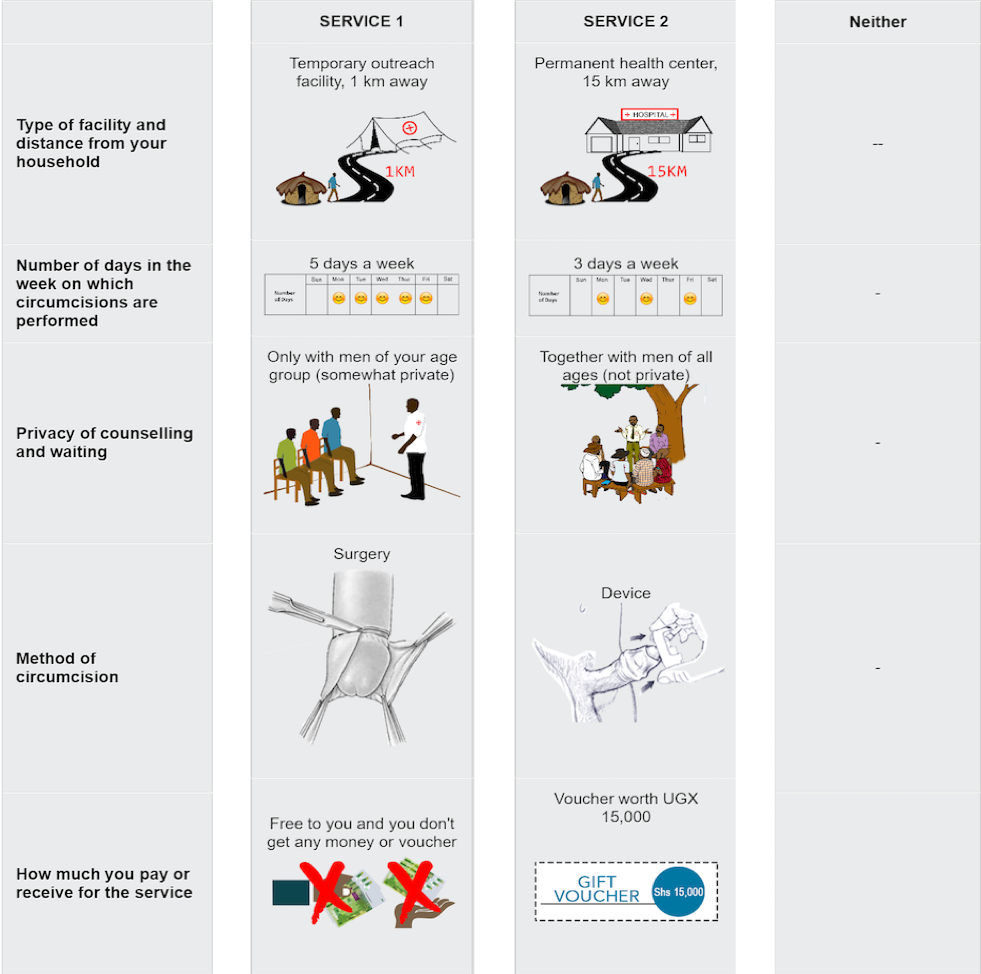
\includegraphics[width=0.78\textwidth]{figures/choice_task.png}
\caption{An example of a choice task.}\label{fig:choicetask}
\end{figure}

\setcounter{section}{3}\setcounter{figure}{0}

\begin{figure}[!htbp]
\centering
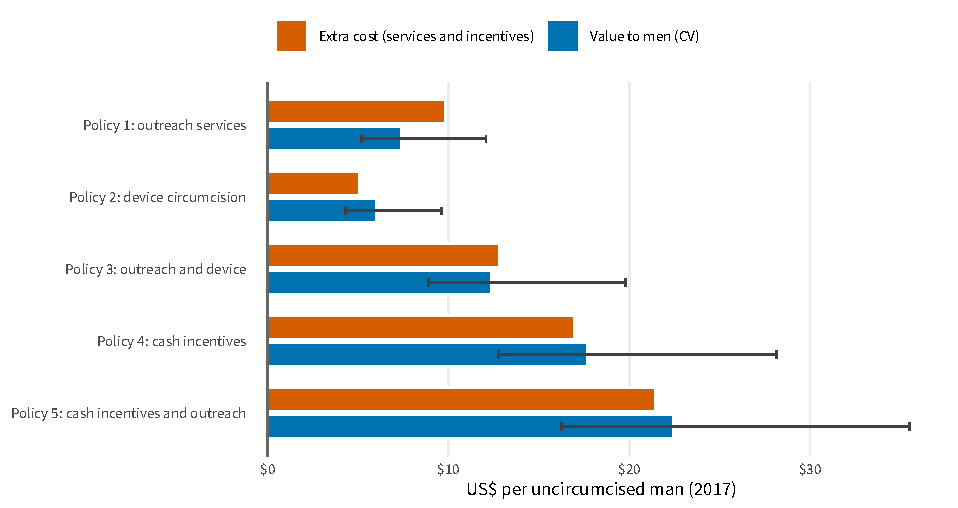
\includegraphics[width=\textwidth]{figures/fig_cv_cost.pdf}
\caption{Compensating variation and incremental cost of each policy per uncircumcised man, compared with the initial state (conditional logit). Whiskers: 95\% Krinsky-Robb intervals for the CV.}\label{fig:cvcost}
\end{figure}

\begin{figure}[!htbp]
\centering
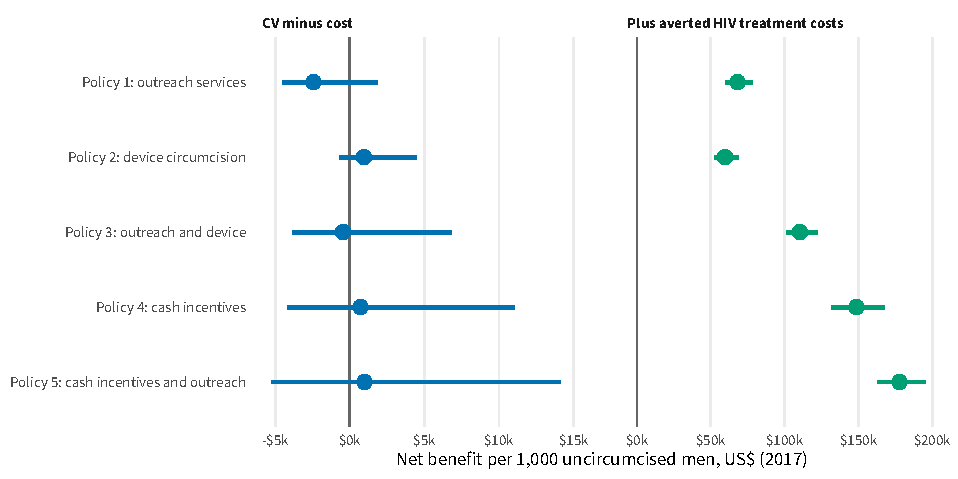
\includegraphics[width=\textwidth]{figures/fig_net_benefit.pdf}
\caption{Net benefit of each policy per 1,000 uncircumcised men, based on the CV alone (left) and including averted HIV treatment costs (right). Points: base case; lines: 95\% Krinsky-Robb intervals. The two panels have different scales.}\label{fig:netbenefit}
\end{figure}

\begin{figure}[!htbp]
\centering
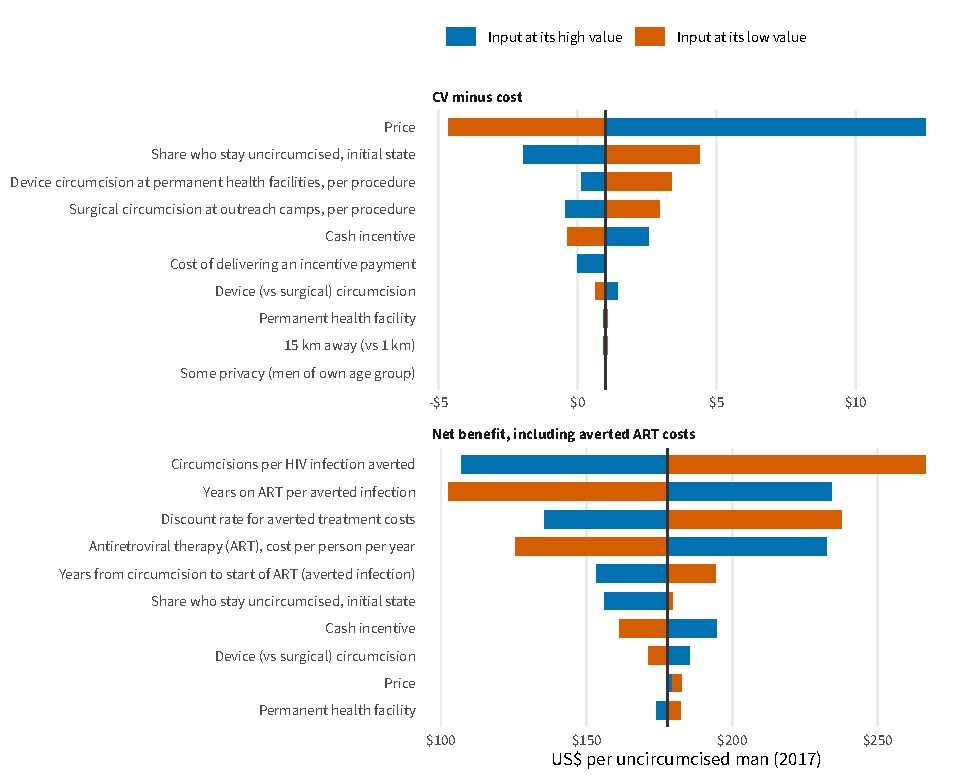
\includegraphics[width=\textwidth]{figures/fig_tornado.pdf}
\caption{One-way sensitivity analyses for cash incentives with outreach services, per uncircumcised man: the ten inputs with the largest effect on the net benefit based on the CV (top) and on the net benefit including averted HIV treatment costs (bottom).}\label{fig:tornado}
\end{figure}

\begin{figure}[!htbp]
\centering
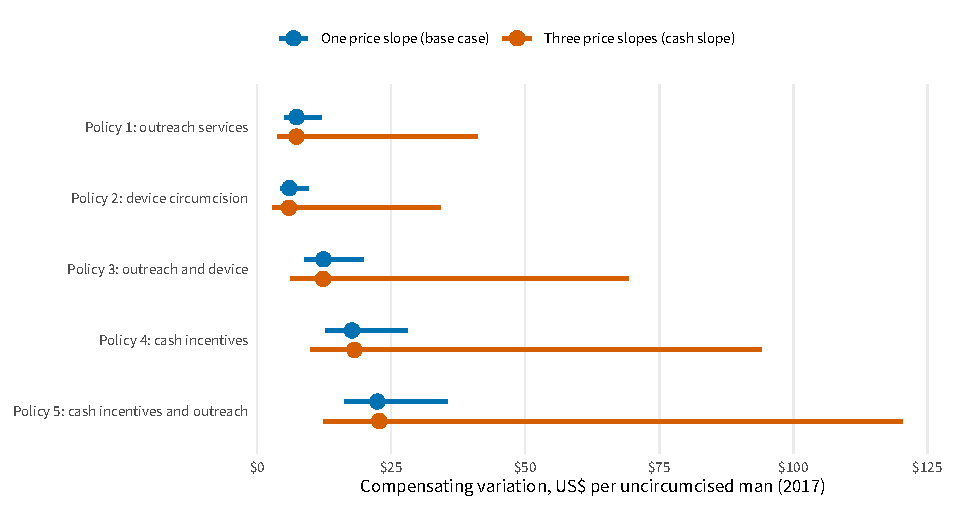
\includegraphics[width=\textwidth]{figures/fig_price_spec.pdf}
\caption{Compensating variation with one price coefficient (base case) and with the cash price coefficient of the model with three price coefficients. Whiskers: 95\% Krinsky-Robb intervals.}\label{fig:pricespec}
\end{figure}

\begin{figure}[!htbp]
\centering
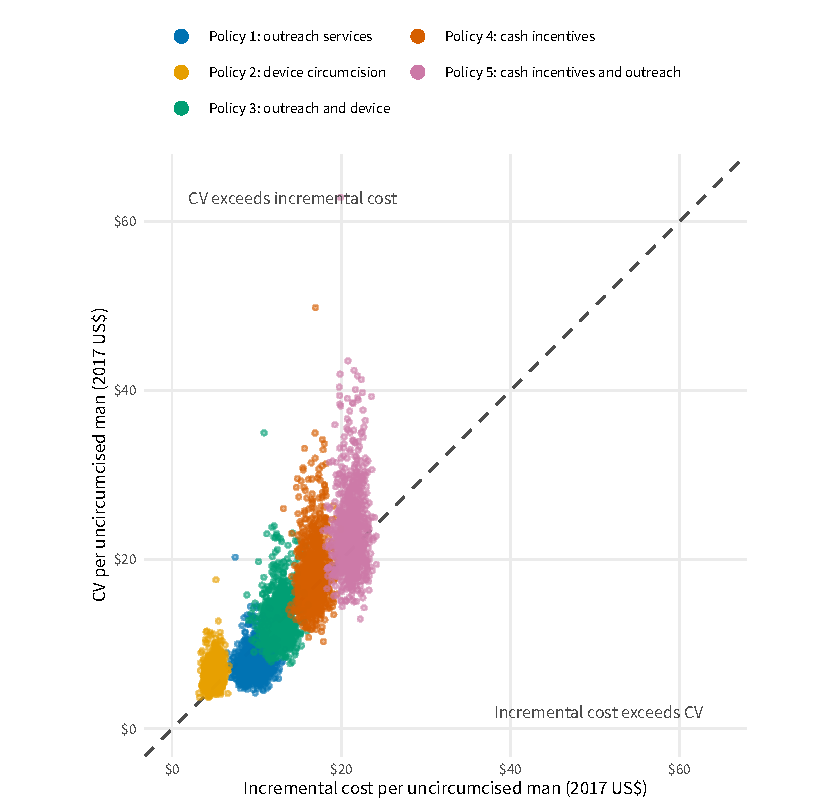
\includegraphics[width=0.78\textwidth]{figures/fig_bc_plane.pdf}
\caption{Benefit-cost plane: incremental cost and CV per uncircumcised man in 800 draws of the probabilistic analysis. Above the dashed line, the CV exceeds the incremental cost.}\label{fig:plane}
\end{figure}

\begin{figure}[!htbp]
\centering
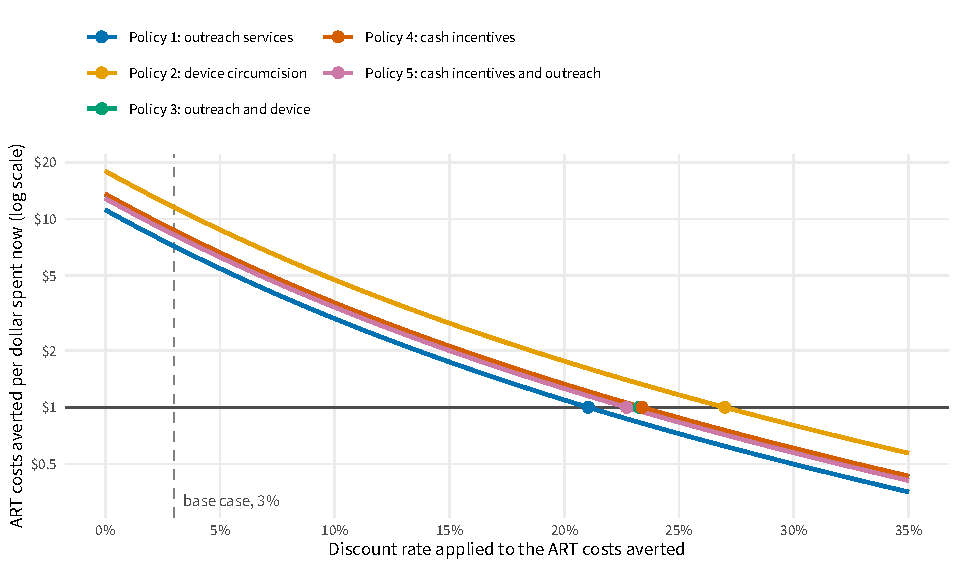
\includegraphics[width=\textwidth]{figures/fig_budget.pdf}
\caption{ART costs averted per dollar spent now, by the discount rate the health budget applies to them (conditional logit). Points: the internal rate of return of each policy, where the ART costs averted just repay the cost. Dashed line: the base-case discount rate.}\label{fig:budget}
\end{figure}

\begin{figure}[!htbp]
\centering
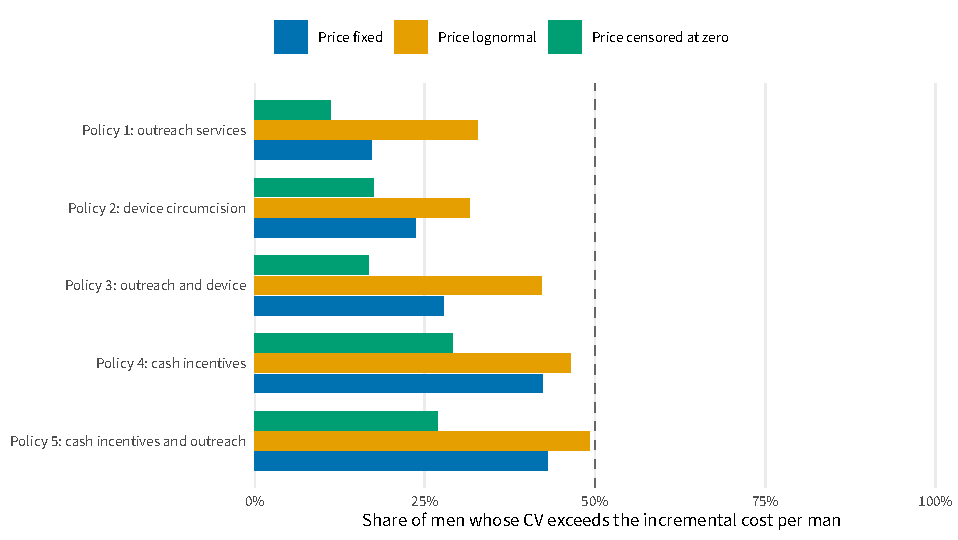
\includegraphics[width=\textwidth]{figures/fig_mixl_share.pdf}
\caption{Share of men whose compensating variation exceeds the incremental cost per uncircumcised man, by policy and distribution of the price coefficient (mixed logit, men with a finite CV). The dashed line marks half of men.}\label{fig:mixlshare}
\end{figure}

\begin{figure}[!htbp]
\centering
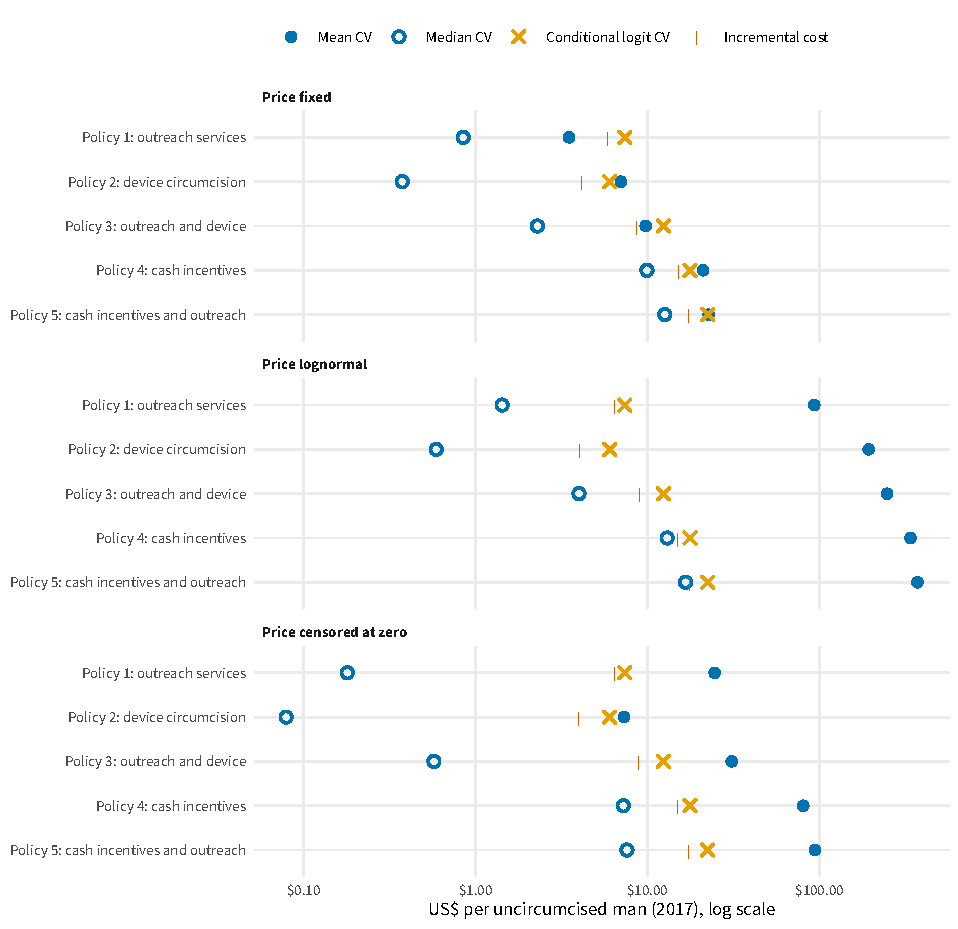
\includegraphics[width=\textwidth]{figures/fig_mixl_cv.pdf}
\caption{Mean and median compensating variation with the mixed logit under three distributions of the price coefficient, with the conditional logit CV and the incremental cost per uncircumcised man (one price coefficient; log scale).}\label{fig:mixlcv}
\end{figure}


% ---- Appendix
\clearpage
\appendix
\section{Compensating variation with a mixed logit}\label{app:cv}
\subsection{Each man's compensating variation}
This appendix derives the results summarised in Section~\ref{sec:cvmixl}. In the mixed logit, men differ in their coefficients, so each man has his own CV. Write man $n$'s utility from alternative $j$ as
\begin{equation}\label{eq:un}
U_{nj} = \lambda_n y_n + V_{nj} + \epsilon_{nj}, \qquad V_{nj} = x_j\boldsymbol{\beta_n},
\end{equation}
where $\lambda_n = -\beta_{price,n}$ is his marginal utility of income. Conditional on $\boldsymbol{\beta_n}$, the errors are Gumbel distributed as before, so his expected maximum utility from a choice set $S$ is
\begin{equation}\label{eq:emax}
E\Big[\max_{j \in S} U_{nj} \;\Big|\; \boldsymbol{\beta_n}\Big] = \lambda_n y_n + \ln \sum_{j \in S} e^{V_{nj}} + C,
\end{equation}
where $C$ is Euler's constant. His CV for a move from $S_0$ to $S_1$ is the payment that leaves this expectation unchanged:
\begin{equation}\label{eq:cvn0}
\lambda_n (y_n - CV_n) + \ln \sum_{j \in S_1} e^{V_{nj}^1} + C = \lambda_n y_n + \ln \sum_{j \in S_0} e^{V_{nj}^0} + C.
\end{equation}
Income and the constant cancel, and solving for $CV_n$ gives
\begin{equation}\label{eq:cvn}
CV_n = CV(\boldsymbol{\beta_n}) = \frac{1}{\lambda_n}\Bigg[\ln \sum_{j \in S_1} e^{V_{nj}^1} - \ln \sum_{j \in S_0} e^{V_{nj}^0}\Bigg] = \frac{\Delta L(\boldsymbol{\beta_n})}{\lambda_n},
\end{equation}
where $\Delta L(\boldsymbol{\beta_n})$ is the change in his log-sum, in units of utility. This is equation~\ref{eq:cv} with his own coefficients in place of the common ones.

\subsection{The mean in the population}
We do not observe $\boldsymbol{\beta_n}$. In the population it follows $f(\boldsymbol{\beta} \mid \Omega)$, so the mean CV in the population is
\begin{equation}\label{eq:ecv}
E[CV] = \int CV(\boldsymbol{\beta})\, f(\boldsymbol{\beta} \mid \Omega)\, d\boldsymbol{\beta}.
\end{equation}
Because $CV(\boldsymbol{\beta})$ is not linear in $\boldsymbol{\beta}$, $E[CV]$ is not the CV at the mean coefficients. In particular, whenever $\lambda$ varies, $E[1/\lambda] > 1/E[\lambda]$ by Jensen's inequality. The integral has no closed form, and with $R$ draws $\boldsymbol{\beta}_r$ from $f(\boldsymbol{\beta} \mid \hat\Omega)$ it is approximated by
\begin{equation}\label{eq:ecvsim}
E[CV] \approx \frac{1}{R}\sum_{r=1}^{R} CV(\boldsymbol{\beta}_r).
\end{equation}

\subsection{Conditioning on each man's choices}
Each man's choices in the survey tell us something about his coefficients. By Bayes' rule, the distribution of $\boldsymbol{\beta}$ among men who made the sequence of choices $y_n$ is\cite{RN89}
\begin{equation}\label{eq:post}
h(\boldsymbol{\beta} \mid y_n, \Omega) = \frac{P(y_n \mid \boldsymbol{\beta})\, f(\boldsymbol{\beta} \mid \Omega)}{P(y_n \mid \Omega)}, \qquad P(y_n \mid \Omega) = \int P(y_n \mid \boldsymbol{\beta})\, f(\boldsymbol{\beta} \mid \Omega)\, d\boldsymbol{\beta},
\end{equation}
with $P(y_n \mid \boldsymbol{\beta})$ from equation~\ref{eq:pseq}. His expected CV, given his choices, is therefore
\begin{equation}\label{eq:cvpost}
E[CV_n \mid y_n] = \int CV(\boldsymbol{\beta})\, h(\boldsymbol{\beta} \mid y_n, \Omega)\, d\boldsymbol{\beta} = \frac{\int CV(\boldsymbol{\beta})\, P(y_n \mid \boldsymbol{\beta})\, f(\boldsymbol{\beta} \mid \Omega)\, d\boldsymbol{\beta}}{\int P(y_n \mid \boldsymbol{\beta})\, f(\boldsymbol{\beta} \mid \Omega)\, d\boldsymbol{\beta}}.
\end{equation}
Using the same $R$ draws in the numerator and the denominator,
\begin{equation}\label{eq:cvpostsim}
E[CV_n \mid y_n] \approx \sum_{r=1}^{R} w_{nr}\, CV(\boldsymbol{\beta}_r), \qquad w_{nr} = \frac{P(y_n \mid \boldsymbol{\beta}_r)}{\sum_{s=1}^{R} P(y_n \mid \boldsymbol{\beta}_s)}.
\end{equation}
Each simulated man $r$ is weighted by how likely he was to make man $n$'s choices. We used \mmcMXsimMen{} draws.

Averaging over the $N = 406$ men in the survey gives the population figure we report:
\begin{equation}\label{eq:cvbar}
\overline{CV} = \frac{1}{N}\sum_{n=1}^{N} E[CV_n \mid y_n] \approx \sum_{r=1}^{R} \omega_r\, CV(\boldsymbol{\beta}_r), \qquad \omega_r = \frac{1}{N}\sum_{n=1}^{N} w_{nr}.
\end{equation}
The second form shows that this is equation~\ref{eq:ecvsim} with the equal weights $1/R$ replaced by $\omega_r$. The population is represented by the 406 conditional distributions pooled together. If the model is correctly specified and the sample represents the population, the average of the conditional distributions over the sample is the population distribution, $\frac{1}{N}\sum_n h(\boldsymbol{\beta} \mid y_n, \Omega) \rightarrow f(\boldsymbol{\beta} \mid \Omega)$,\cite{RN89} so $\overline{CV}$ and $E[CV]$ estimate the same quantity. We computed both; a large difference between them would point to a misspecified mixing distribution.

\subsection{Median, share gaining, uptake and calibration}
The same weights give the median CV, the value $m$ that solves
\begin{equation}\label{eq:median}
\sum_{r=1}^{R} \omega_r\, \mathbf{1}\big[CV(\boldsymbol{\beta}_r) \le m\big] = \frac{1}{2},
\end{equation}
and the share of men whose CV exceeds the incremental cost per man, $\Delta C$ (equation~\ref{eq:cost}),
\begin{equation}\label{eq:gain}
G = \sum_{r=1}^{R} \omega_r\, \mathbf{1}\big[CV(\boldsymbol{\beta}_r) > \Delta C\big].
\end{equation}
Choice probabilities are averaged in the same way, $\bar P_j(S) = \sum_r \omega_r P_j(S \mid \boldsymbol{\beta}_r)$, and take the place of the conditional logit probabilities in equations~\ref{eq:cost} and~\ref{eq:nb}. The opt-out constant is calibrated as in equation~\ref{eq:calibration}, with one shift $\hat a$ for all men, chosen so that $\sum_r \omega_r P_0(S_0 \mid \boldsymbol{\beta}_r, \hat a) = S$.

\subsection{The plug-in estimate}
A common shortcut is to compute each man's CV at his posterior mean coefficients:
\begin{equation}\label{eq:plugin}
CV(\bar{\boldsymbol{\beta}}_n), \qquad \bar{\boldsymbol{\beta}}_n = E[\boldsymbol{\beta} \mid y_n] \approx \sum_{r=1}^{R} w_{nr}\, \boldsymbol{\beta}_r.
\end{equation}
Because $CV(\boldsymbol{\beta})$ is not linear in $\boldsymbol{\beta}$, $CV(\bar{\boldsymbol{\beta}}_n)$ is not $E[CV_n \mid y_n]$. When $\lambda$ is fixed, the difference comes only from the log-sum and is usually small. When $\lambda$ varies, $1/\bar\lambda_n$ understates the posterior mean of $1/\lambda$, and the difference can be large. We report this plug-in estimate for comparison.

\subsection{The distribution of the marginal utility of income}
The distribution of $\lambda$ decides whether the mean CV is well behaved. From equation~\ref{eq:cvn}, $E[CV] = E[\Delta L(\boldsymbol{\beta})/\lambda]$. With a fixed $\lambda$ this is $E[\Delta L]/\lambda$. Now take a policy that does not change what men pay, such as outreach services or device circumcision. Its $\Delta L$ does not involve the price coefficient, and because the coefficients are independent, $\Delta L$ and $\lambda$ are independent, so that
\begin{equation}\label{eq:ecvindep}
E[CV] = E[\Delta L]\; E\Big[\frac{1}{\lambda}\Big].
\end{equation}
With a log-normal price coefficient, $\lambda = \exp(\mu + \sigma\zeta)$, so $1/\lambda = \exp(-\mu - \sigma\zeta)$, where $-\mu - \sigma\zeta \sim \mathcal{N}(-\mu, \sigma^2)$. For any $X \sim \mathcal{N}(a, s^2)$, $E[e^X] = e^{a + s^2/2}$, so
\begin{equation}\label{eq:invlambda}
E\Big[\frac{1}{\lambda}\Big] = \exp\Big(-\mu + \frac{\sigma^2}{2}\Big) = \frac{1}{\lambda_{med}}\exp\Big(\frac{\sigma^2}{2}\Big),
\end{equation}
where $\lambda_{med} = \exp(\mu)$ is the median of $\lambda$. Substituting equation~\ref{eq:invlambda} into equation~\ref{eq:ecvindep}, the mean CV is $E[\Delta L]/\lambda_{med}$, the CV of a man with the median price coefficient, multiplied by $\exp(\sigma^2/2)$. The factor grows quickly with $\sigma$: it is 1.6 at $\sigma = 1$ and 7.4 at $\sigma = 2$. With a censored normal price coefficient, $\lambda = \max(0, -\mu - \sigma\zeta)$, and a share $\Phi(\mu/\sigma)$ of men have $\lambda = 0$. Their CV is unbounded, so $E[CV]$ does not exist.\cite{DalyHessTrain2012} For this specification we report the mean and median CV among men with $\lambda > 0$, and the share with $\lambda = 0$.

\end{document}
